\documentclass[11pt]{article}

% ===== Geometry & typography =====
\usepackage[margin=1in,letterpaper]{geometry}
\usepackage[T1]{fontenc}
\usepackage[utf8]{inputenc}
\usepackage{lmodern}
\usepackage{microtype}
\usepackage{setspace}\setstretch{1.05}
\setlength{\parskip}{0.55em}
\setlength{\parindent}{0pt}

% ===== Math =====
\usepackage{amsmath,amssymb,amsfonts,amsthm,mathtools,bm}

% ===== Figures, tables, code =====
\usepackage{graphicx}
\usepackage{booktabs,array,multirow,longtable}
\usepackage{caption}\captionsetup{font=small,labelfont=bf}
\usepackage{subcaption}
\usepackage{listings}
\usepackage{enumitem}
\setlist{topsep=2pt,itemsep=2pt}
\usepackage{xcolor}
\usepackage{colortbl}
\usepackage{float}
\usepackage{tcolorbox}
\tcbuselibrary{breakable,skins}

\definecolor{cb}{HTML}{1f77b4}
\definecolor{cr}{HTML}{d62728}
\definecolor{cg}{HTML}{2ca02c}
\definecolor{cy}{HTML}{8c6d31}
\definecolor{cv}{HTML}{9467bd}
\definecolor{cgray}{HTML}{555555}
\definecolor{codebg}{RGB}{248,248,248}

% ===== Hyperlinks =====
\usepackage[hidelinks]{hyperref}
\usepackage{cleveref}

% ===== Custom boxes =====
\newtcolorbox{analogy}[1][]{enhanced,breakable,
  colback=cy!8,colframe=cy!60!black,boxrule=0.6pt,
  arc=2pt,left=8pt,right=8pt,top=4pt,bottom=4pt,
  title={\textbf{Analogy:} #1},fonttitle=\small,coltitle=cy!50!black,
  attach boxed title to top left={xshift=8pt,yshift=-6pt},
  boxed title style={colback=cy!18,colframe=cy!60!black,boxrule=0.4pt}}

\newtcolorbox{plainenglish}[1][]{enhanced,breakable,
  colback=cb!6,colframe=cb!60!black,boxrule=0.6pt,
  arc=2pt,left=8pt,right=8pt,top=4pt,bottom=4pt,
  title={\textbf{Plain English:} #1},fonttitle=\small,coltitle=cb!50!black,
  attach boxed title to top left={xshift=8pt,yshift=-6pt},
  boxed title style={colback=cb!15,colframe=cb!60!black,boxrule=0.4pt}}

\newtcolorbox{walkthrough}[1][]{enhanced,breakable,
  colback=cg!6,colframe=cg!60!black,boxrule=0.6pt,
  arc=2pt,left=8pt,right=8pt,top=4pt,bottom=4pt,
  title={\textbf{Walkthrough:} #1},fonttitle=\small,coltitle=cg!50!black,
  attach boxed title to top left={xshift=8pt,yshift=-6pt},
  boxed title style={colback=cg!15,colframe=cg!60!black,boxrule=0.4pt}}

\newtcolorbox{definition}[1][]{enhanced,breakable,
  colback=cv!6,colframe=cv!60!black,boxrule=0.6pt,
  arc=2pt,left=8pt,right=8pt,top=4pt,bottom=4pt,
  title={\textbf{Definition:} #1},fonttitle=\small,coltitle=cv!50!black,
  attach boxed title to top left={xshift=8pt,yshift=-6pt},
  boxed title style={colback=cv!15,colframe=cv!60!black,boxrule=0.4pt}}

\newtcolorbox{punchline}{enhanced,breakable,
  colback=cr!6,colframe=cr!60!black,boxrule=0.8pt,
  arc=2pt,left=8pt,right=8pt,top=6pt,bottom=6pt}

% ===== Math shorthands =====
\newcommand{\R}{\mathbb{R}}
\newcommand{\E}{\mathbb{E}}
\newcommand{\Prb}{\mathbb{P}}
\newcommand{\argmax}{\operatorname*{arg\,max}}
\newcommand{\bel}{\mathbf{b}}

% ===== Code style =====
\lstset{
  basicstyle=\ttfamily\footnotesize,
  backgroundcolor=\color{codebg},
  frame=single,
  breaklines=true,
  numbers=left,
  numberstyle=\tiny\color{gray},
  keywordstyle=\color{cb},
  commentstyle=\color{cgray}\itshape,
  stringstyle=\color{cr},
  showstringspaces=false,
  xleftmargin=1.5em,
}

% ===== Title =====
\title{
  \LARGE\textbf{Walkthrough Companion}\\[6pt]
  \large Regime-Switching Asset Allocation via a POMDP\\[2pt]
  \normalsize\itshape A plain-language guide to the project, the paper, the experiments, and the slides
}
\author{
  Dario Blanco Morales \quad Even Hogberget \quad Kyle David Ledda-Lewaren \quad Taka Khoo \\[2pt]
  \small ENGS 177: Decision Making Under Uncertainty, Spring 2026 \\
  \small Thayer School of Engineering, Dartmouth College
}
\date{May 2026}

\begin{document}

\maketitle

\vspace{-1em}
\begin{plainenglish}[What is this document?]
This is a long, plain-language companion to our term project. Read it instead of (or alongside) the 11-page class report \texttt{report.pdf} and the 38-page \texttt{extended\_report.pdf} if you want every term defined, every figure explained, every experiment narrated, and every result placed in the bigger picture, with analogies, real-world examples, and as little math as possible. It does not replace the formal documents. It makes them accessible.

If you are presenting the slides or sitting in on the talk, the last chapter is a guide to the 15-frame condensed deck.
\end{plainenglish}

\tableofcontents
\bigskip\hrule

%======================================================================
\part{Setting the Scene}
%======================================================================

%====================================================================
\section{What problem are we even solving?}
%====================================================================

\subsection{The everyday version}

You are 25 years old. You have a job. Every month, after rent and groceries, you have some leftover money that you want to grow over time so that one day you can retire, buy a house, send a kid to college, or just sleep well at night. You decide to invest it.

The simplest piece of advice you have ever heard is some version of: ``put 60\% of your savings in stocks and 40\% in bonds, and forget about it.'' That recipe is called the \textbf{60/40 portfolio}. It has been the textbook starting point for ordinary savers for half a century. Universities teach it. Financial advisors recommend it. Target-date retirement funds default to something close to it.

The promise is two-fold. Stocks grow your money over the long run, because companies grow. Bonds protect you when stocks crash, because investors flee to safety. Add them together and you get growth-with-a-cushion. Year in, year out, it just sort of works.

Until it doesn't.

\subsection{The 2022 problem}

In 2022, the U.S.\ stock market (measured by the S\&P~500) fell about 18\%. That alone would have been a normal bad year. But that same year, U.S.\ aggregate bonds (the boring stuff that is supposed to act as a cushion) \emph{also} fell, by about 13\%. Both legs of the textbook 60/40 portfolio went down together. The standard textbook portfolio lost about 17\% in a single year, one of its worst years on record.

\begin{punchline}
\centering\large
The thing 60/40 is supposed to protect against (a coordinated equity-and-bond sell-off) is exactly what happened in 2022. The recipe failed at its only job.
\end{punchline}

Why? Because the world had changed. Inflation came roaring back. The Federal Reserve raised interest rates aggressively to fight it. High inflation hurts stocks (it eats into corporate earnings) \emph{and} high interest rates hurt bonds (because new bonds become more attractive, making old bonds worth less). The two ``protections'' moved together because the same force was hurting both at once. The diversification story broke down.

\subsection{The research question, in everyday language}

So we asked: \emph{can we do better?} Not better in some flashy ``beat-the-market'' sense, but better in a disciplined, principled way:

\begin{itemize}
  \item Can we build a system that watches the broader economic environment, recognises when conditions are \emph{usually} dangerous, and tilts the portfolio toward safer assets before the danger arrives?
  \item Can we do this with publicly-available data, no insider information, and rules that anyone could write down and audit?
  \item And critically: can we tell whether our system actually \emph{works}, not just on the period we designed it on, but on a long out-of-sample stretch of history?
\end{itemize}

\subsection{The research question, in the language of the course}

In ENGS~177 language, we are looking at a \emph{sequential decision problem under partial information}. Every month we have to decide a portfolio allocation. The decision affects future wealth. We don't directly see the ``regime'' the economy is in, we only see noisy indicators of it. The decision now affects what beliefs we will hold next month. This is the textbook signature of a \textbf{POMDP (Partially Observable Markov Decision Process)}.

Section~\ref{sec:terms} unpacks every term in that sentence in plain English.

%====================================================================
\section{Who are we and why are we doing this?}
%====================================================================

We are four Dartmouth Thayer students in Professor Wesley Marrero's Spring 2026 ENGS~177 course on \emph{Decision Making Under Uncertainty}: Dario Blanco Morales, Even Hogberget, Kyle David Ledda-Lewaren, and Taka Khoo.

\subsection{Why this project type}

The course required either a \emph{New Application} project (use the course tools on a problem they weren't built for) or a \emph{Methods} project (extend the tools themselves). We picked New Application. The asset-allocation problem is a great laboratory because:

\begin{itemize}
  \item Public real-world data is plentiful (free FRED + Yahoo Finance).
  \item The decision is genuinely repeated (monthly rebalance), so dynamic programming actually applies.
  \item It connects directly to several lectures: Markov chains, Bayesian filters, MDPs, POMDPs, value iteration, policy iteration, multi-armed bandits, Monte Carlo, TD learning.
  \item There is a long, contentious literature: people have been claiming for decades that regime-switching beats static allocation. We get to test it ourselves.
\end{itemize}

\subsection{The honest motivation}

We are not trying to invent a strategy you should put your savings into. We are trying to understand whether a principled, fully decision-theoretic approach can clear the practitioner-consensus bar. If we don't beat 60/40 (and spoiler: in our headline configuration we don't), we want to know \emph{exactly which methodological choice} drives the failure. That's the real contribution of this project, not the strategy, but the diagnostic of why the strategy underperforms, with experiments that each isolate one choice.

\begin{plainenglish}[Why publish a project that doesn't beat the benchmark?]
Most published regime-switching papers report Sharpe wins. Many of them survive only inside a specific tuning of observations, training window, and risk aversion. Our project is unusual in that we publish the negative headline and then \emph{decompose} it: which knob, if you flipped just that one, would reverse the verdict? That makes the project falsifiable, comparable, and honest, properties we value more than a flashy number.
\end{plainenglish}

%======================================================================
\part{All the Words}
%======================================================================

%====================================================================
\section{Every term, defined plainly}\label{sec:terms}
%====================================================================

This whole project lives in a tower of jargon. Most of it is unnecessary to understand the story; some of it is essential. Here is every term you need, in roughly the order it first appears, defined in plain English first and then formally.

\subsection{Financial terms}

\begin{definition}[Portfolio]
A list of how much of each asset you own. In our project a ``portfolio'' is just two numbers: the fraction in stocks (SPY) and the fraction in bonds (AGG), which must add to 100\%. So ``60/40'' means 60\% stocks and 40\% bonds.
\end{definition}

\begin{definition}[Return]
The percentage change in the price of an asset over a fixed period (we use one month). If SPY was \$400 at the start of January and \$408 at the start of February, the January return was $+2\%$. A negative return means a loss.
\end{definition}

\begin{definition}[Rebalance]
The act of changing your portfolio weights. If you're at 60/40 and stocks rose so you drifted to 65/35, ``rebalancing'' is selling some stocks and buying bonds to get back to your target weights. We rebalance monthly.
\end{definition}

\begin{definition}[Benchmark]
A reference portfolio you compare yours against. Ours is the static 60/40, the textbook default. ``Beating the benchmark'' means delivering more return per unit of risk than 60/40.
\end{definition}

\subsection{Risk metrics}

\begin{definition}[CAGR, Compound Annual Growth Rate]
The single annual growth rate that, compounded, takes your starting value to your ending value over the full period. Captures \emph{total} growth, ignoring the bumpiness of the path.
\end{definition}

\begin{definition}[Volatility]
The annualised standard deviation of monthly returns. A measure of how bumpy the ride is. A portfolio with 10\% volatility wiggles around its average return by typically $\pm 10\%$ over a year.
\end{definition}

\begin{definition}[Sharpe ratio]
\emph{Excess return divided by volatility.} Tells you how much extra return you got per unit of risk you took. The single most-cited risk-adjusted performance metric. Higher is better; 1.0 is good, 1.5 is great, 2.0+ is rare-air territory.
\end{definition}

\begin{definition}[Sortino ratio]
Like Sharpe, but only penalises \emph{downside} volatility (volatility on losing months only). The intuition: who cares if your returns are bumpy in the good direction? Sortino captures that asymmetry.
\end{definition}

\begin{definition}[Max drawdown]
The biggest peak-to-trough percentage loss you would have suffered if you'd invested at the worst possible moment in the sample. ``$-30\%$ max drawdown'' means at the worst moment in the backtest, you were 30\% down from your previous high-water mark. This is the ``how badly will I want to throw up'' metric.
\end{definition}

\begin{definition}[Calmar ratio]
CAGR divided by max drawdown. ``How much return did I get per unit of pain?'' Higher is better.
\end{definition}

\begin{definition}[Turnover]
How much trading you do, measured as the $L_1$ change in portfolio weights from month to month, averaged over the sample. Higher turnover means more trading costs in real life.
\end{definition}

\subsection{Course-specific terms}

\begin{definition}[State]
A snapshot of all the information that matters for future decisions. In a board game, the state is the current position of all pieces. In our project, the state is which \emph{regime} the economy is in.
\end{definition}

\begin{definition}[Action]
A decision you make. In our project, an action is a portfolio weight: pick one of $\{0/100, 20/80, 40/60, 60/40, 80/20, 100/0\}$.
\end{definition}

\begin{definition}[Reward]
The immediate payoff after taking an action in a state. In our project the reward is a \emph{utility} of next month's portfolio return, minus a small transaction cost.
\end{definition}

\begin{definition}[Transition matrix $T(s' \mid s)$]
The probability of moving from state $s$ to state $s'$ in one step. ``If we are in bull regime today, what's the chance we'll be in bear regime next month?''
\end{definition}

\begin{definition}[Discount factor $\lambda$]
A number between 0 and 1 that says how much you value future rewards relative to today's. $\lambda = 0.99$ means a reward next month is worth 99\% of the same reward this month. Smaller $\lambda$ makes you myopic; larger makes you patient.
\end{definition}

\begin{definition}[Policy $\pi$]
A rule that maps states (or beliefs) to actions. ``In bull regime, pick action $a_1$; in bear regime, pick action $a_2$.''
\end{definition}

\begin{definition}[Value function $V^*(s)$]
The expected total discounted reward you would earn starting in state $s$ and following the optimal policy forever. ``If we end up in bull regime now, what's the long-run discounted expected utility?''
\end{definition}

\begin{definition}[Q-function $Q^*(s,a)$]
Like the value function, but also conditioning on the action you take first. ``If we end up in bull regime and choose action $a$, then act optimally afterwards, what's the expected total discounted utility?''
\end{definition}

\begin{definition}[MDP, Markov Decision Process]
A formal model with a state, an action, a transition matrix, a reward, and a discount factor. The defining ``Markov'' property: the future depends only on the current state, not the path that got you there.
\end{definition}

\begin{definition}[POMDP, Partially Observable MDP]
An MDP where you don't directly see the state. You only see noisy \emph{observations} that are statistically related to the state. The right thing to track is now a probability distribution over states, called a \emph{belief}.
\end{definition}

\begin{definition}[HMM, Hidden Markov Model]
A statistical model of a system that has a hidden state evolving as a Markov chain and produces observations that depend on the current hidden state. Used in our project to model how the latent economic regime produces the noisy macro observations we actually see.
\end{definition}

\begin{definition}[Belief $\bel_t$]
A probability vector over the hidden states at time $t$. ``We think there's a 78\% chance we're in bull regime and a 22\% chance we're in bear regime, given everything we've observed so far.''
\end{definition}

\begin{definition}[Bayes filter]
The recursive algorithm that updates your belief given a new observation. ``Yesterday I was 78\% bull. Today I saw VIX jump to 35. My updated belief is 7\% bull, 93\% bear.''
\end{definition}

\begin{definition}[Value iteration (VI)]
An algorithm that solves the Bellman equation by repeatedly applying the Bellman operator until the value function stops changing. Slow but conceptually simple.
\end{definition}

\begin{definition}[Policy iteration (PI)]
An algorithm that alternates between (i) evaluating a fixed policy by solving a linear system and (ii) improving the policy greedily. Faster than VI for small problems; uses exact policy evaluation.
\end{definition}

\begin{definition}[QMDP]
A simple approximation for POMDPs. Solve the underlying \emph{fully-observable} MDP for $Q^*(s, a)$. At decision time, given belief $\bel$, choose the action $a$ that maximises $\sum_s \bel(s) Q^*(s, a)$. Treats the belief as if it were a probability over what the ``true state'' is going to be revealed to be next.
\end{definition}

\begin{definition}[Utility]
A function $U(\cdot)$ that maps a numerical return into a number representing how much you actually \emph{value} that return. Concave utility (like our CRRA) means a \$100 gain feels less good than a \$100 loss feels bad, you are \emph{risk averse}.
\end{definition}

\begin{definition}[CRRA utility]
Constant Relative Risk Aversion utility: $U(r) = \frac{(1+r)^{1-\gamma}}{1-\gamma}$. The parameter $\gamma$ tunes how risk-averse you are: $\gamma = 0$ means you only care about expected return; $\gamma \to \infty$ means you only care about avoiding losses.
\end{definition}

\subsection{Empirical baseline strategies (one-liners)}

We benchmark QMDP against eleven other strategies. Here is what each one does in one sentence:

\begin{itemize}
  \item \textbf{Static 60/40.} Hold 60\% stocks and 40\% bonds, always.
  \item \textbf{Equal weight.} Hold 50\% stocks and 50\% bonds, always.
  \item \textbf{Inverse volatility.} Put more weight on the asset that has been less volatile recently.
  \item \textbf{Risk parity (ERC).} Pick weights so that each asset contributes equally to overall portfolio risk.
  \item \textbf{Mean-variance + Ledoit--Wolf.} Solve the classical Markowitz optimisation using a regularised covariance matrix.
  \item \textbf{Faber 10-month SMA.} Hold the asset if its price is above its 10-month moving average; else go to cash.
  \item \textbf{Time-series momentum.} Hold the asset if its 12-month return was positive; weight by sign.
  \item \textbf{Vol-target 60/40.} Run 60/40 but scale leverage up or down to hit a target volatility.
  \item \textbf{Myopic 12-month.} Pick the allocation that would have maximised the last 12 months of return.
  \item \textbf{HMM-conditional MV.} Solve Markowitz against belief-weighted regime-conditional return moments.
  \item \textbf{Black--Litterman + HMM.} Combine equilibrium market priors with HMM-derived views, then do mean-variance.
\end{itemize}

%====================================================================
\section{The pipeline in five analogies}
%====================================================================

The full system has five conceptual stages. Each one has a one-paragraph analogy in plain English.

\subsection{Analogy 1: the doctor (this whole project, in one image)}

\begin{analogy}[The doctor and the patient]
You are a doctor. Your patient is the stock-bond market. Every month at the check-up (rebalance) you must prescribe a treatment (portfolio weights). The patient is either \emph{healthy} (bull regime) or \emph{sick} (bear regime), but you cannot examine their internal state directly, you only see symptoms (VIX level, term spread, financial-stress indices). Different treatments work better in different states. Your job: read the symptoms, infer the latent state, prescribe accordingly.
\end{analogy}

That is literally a POMDP. The doctor's job is well-defined: maintain a belief about the patient's state given the symptoms seen so far, and pick the treatment that maximises expected long-run health.

\subsection{Analogy 2: the casino dealer (the HMM)}

\begin{analogy}[The dealer secretly switching decks]
Imagine a poker dealer who, between rounds, secretly swaps between two decks of cards. Deck~A has lots of high cards (the bull regime: positive expected returns). Deck~B has lots of low cards (the bear regime: negative). You never see which deck is in play. You only see the cards.
\end{analogy}

The deck-switching probabilities are the \textbf{transition matrix $T$}. The card distribution under each deck is the \textbf{emission distribution} (in our project: a Gaussian). The algorithm that figures out, from a long stream of observed cards, what each deck must look like and how often the dealer switches is called \textbf{Baum--Welch}, it is the EM algorithm specialised to HMMs.

For our project: the ``cards'' are monthly observations of (VIX, term spread). The fitted transition matrix is roughly $\begin{psmallmatrix} 0.96 & 0.04 \\ 0.06 & 0.94 \end{psmallmatrix}$. Both regimes are \emph{very sticky}, in any given month there's only a 4--6\% chance the dealer switches decks.

\subsection{Analogy 3: updating your guess about which deck is in play (the Bayes filter)}

\begin{analogy}[Updating after each card]
After every card, you update your guess about which deck is active. You have a prior belief (``I think it's 70\% Deck~A based on what I've seen so far''). The dealer might have just switched, so you adjust for that possibility (\emph{predict step}). Then a card comes out. If it's high, it boosts your suspicion of Deck~A; if low, of Deck~B (\emph{update step}).
\end{analogy}

The Bayes filter is the formal version of that updating. For our HMM, the predict step is
\[
\hat b_t(s') = \sum_s T(s' \mid s)\, b_{t-1}(s)
\]
and the update step is
\[
b_t(s') \propto O(\mathbf{o}_t \mid s')\, \hat b_t(s').
\]

A single observation of VIX$=35$ can flip a 70/30 ``bull'' prior into a 7/93 ``bear'' posterior. That responsiveness is the entire point.

\subsection{Analogy 4: the dealer dealt face-up (the underlying MDP)}

\begin{analogy}[Cards face-up]
Suppose the dealer turned the decks face-up, you can see at every moment which deck is in use. What's the best action in each deck? That's the easier sub-problem. Solve the Bellman equation by value iteration or policy iteration. The answer is a small table: ``in Deck~A do X; in Deck~B do Y.''
\end{analogy}

This is the \emph{fully-observable MDP} hidden inside our POMDP. We can solve it cleanly because the state space is small (just 2 regimes) and the action space is small (just 6 allocations). Both Value Iteration and Policy Iteration give the same answer (they have to, the Bellman operator is a contraction); we run both as a sanity check and they agree to $2.6 \times 10^{-6}$ component-wise.

\subsection{Analogy 5: the dealer secretly whispers a probability (QMDP)}

\begin{analogy}[The whisper]
Suppose the dealer privately whispers in your ear: ``You're in Deck~A with probability $b(A)$ and Deck~B with probability $b(B)$.'' What's the best action under that whisper? Pick the action that maximises the average of $Q^*(s, a)$ weighted by the whispered probabilities:
\[
\pi_{\mathrm{QMDP}}(\bel) = \argmax_a \sum_s b(s)\, Q^*(s, a).
\]
\end{analogy}

That's QMDP. It is the simplest approximate POMDP solver and it is exact when the belief is concentrated on a single state. Its main weakness is that it cannot motivate the agent to take \emph{information-gathering} actions, but in our setting no action affects observability (we see VIX regardless of how we allocate), so the weakness does not bind here.

%======================================================================
\part{The Data, What Are We Actually Looking At?}
%======================================================================

%====================================================================
\section{What's in the panel and where it comes from}
%====================================================================

All inputs are public. Nothing in this project requires an API key, a paid subscription, or insider information. The full dataset is committed in the repository under \texttt{data/raw/}.

\subsection{The two assets}

\begin{itemize}
  \item \textbf{SPY}, a fund that tracks the S\&P~500 (the 500 largest U.S.\ public companies). When SPY goes up, U.S.\ equity markets are doing well.
  \item \textbf{AGG}, a fund that tracks the U.S.\ aggregate bond market (a broad mix of Treasury, mortgage, and corporate bonds). When AGG goes up, U.S.\ bond prices are rising (typically because interest rates are falling).
\end{itemize}

We pull daily prices for both from Yahoo Finance, take the last price each month, and compute monthly log-returns. The AGG fund was launched in September~2003, which sets the start of our panel.

\subsection{The headline observations}

Our HMM's job is to figure out the current regime by watching macro-financial indicators. We feed it two ``headline'' observation channels:

\begin{itemize}
  \item \textbf{VIX} (FRED series \texttt{VIXCLS}). The CBOE Volatility Index. Measures the market's expectation of S\&P~500 volatility over the next 30 days, derived from the prices of options. ``Fear gauge.'' Normally between 12 and 20. In a crisis, it spikes above 40 (October 2008: 80; March 2020: 82).
  \item \textbf{10Y--3M Treasury spread} (FRED series \texttt{T10Y3M}). The yield on 10-year Treasury bonds minus the yield on 3-month Treasury bills. ``Yield curve slope.'' Normally positive (long-term loans should pay more than short-term loans). When it goes negative (an ``inverted yield curve''), it has historically predicted recession within 6--18 months.
\end{itemize}

Together these two are supposed to capture both market fear (VIX) and macro expectations (term spread).

\subsection{Why two more channels matter so much (the Unlock 1 punchline)}

Here is the spoiler we will earn in Section~\ref{sec:unlocks}: VIX and the term spread by themselves are not enough to make a regime-aware policy actually differ between bull and bear states. They both rise during \emph{equity} crises but miss other kinds of stress. So we also fetch:

\begin{itemize}
  \item \textbf{NFCI, Chicago Fed National Financial Conditions Index} (FRED: \texttt{NFCI}). A weekly composite of 105~separate financial-stress indicators across equity, bond, money-market, and shadow-banking systems. Higher = tighter financial conditions. Goes up sharply in 2008, 2020, and (importantly) 2022.
  \item \textbf{STLFSI4, St.\ Louis Fed Financial Stress Index} (FRED: \texttt{STLFSI4}). A weekly composite of 18 different financial-stress indicators. Like NFCI but with a different aggregation method, they cross-validate each other.
\end{itemize}

Adding these two changes everything for the policy, as we'll see in Section~\ref{sec:unlocks}.

\subsection{The other extension channels}

We pull six more series for the ``kitchen sink'' cohort experiment:

\begin{itemize}
  \item \textbf{T10Y2Y} (FRED), alternate yield-curve slope.
  \item \textbf{UMCSENT} (FRED), University of Michigan consumer-sentiment index. Households' subjective view of the economy.
  \item \textbf{ICSA} (FRED), initial unemployment claims, weekly. A high-frequency labour-market signal.
  \item \textbf{DTWEXBGS} (FRED), trade-weighted broad dollar index. Captures global flight-to-USD.
  \item \textbf{DCOILWTICO} (FRED), WTI crude oil price. Captures supply-side shocks.
  \item \textbf{DFF} (FRED), effective federal funds rate. The Federal Reserve's policy stance.
\end{itemize}

\subsection{What we use for validation but never for training}

\begin{itemize}
  \item \textbf{NBER recession dates} (FRED: \texttt{USREC}). The National Bureau of Economic Research's official, retrospectively-dated U.S.\ recession periods. We \emph{never} feed these to the model. We only use them at the end, to qualitatively check whether the HMM's inferred ``bear regime'' bracket lines up with the recessions the NBER eventually labelled.
\end{itemize}

\subsection{Putting it all together}

The script \texttt{src/data/fetch\_data.py} downloads each series, resamples daily series to month-end, aligns everything by date, and writes a single CSV: \texttt{data/processed/monthly.csv}. After alignment, this file has 272 rows (one per month from October~2003 to April~2026) and 13 columns (10 observation channels + the NBER flag + 2 asset returns).

\begin{walkthrough}[Why 272 rows and not more?]
We have plenty of decades of VIX data, but AGG was launched in September~2003. To keep the panel clean and consistent, we use the longest window for which every series is simultaneously available: October~2003 onward. That gives us 272 months. After dropping the first row (which we use as the prior), 271 usable months.
\end{walkthrough}

%======================================================================
\part{The Pipeline, How a Decision Is Made Each Month}
%======================================================================

%====================================================================
\section{The pipeline diagram, walked through box-by-box}
%====================================================================

Figure~\ref{fig:pipeline} (in the class report) shows the full pipeline as a flowchart. Let's walk through it slowly.

\subsection{Step 1: raw data ingest}

\textbf{Box.} ``FRED + Yahoo'' $\to$ ``Monthly panel.''

\textbf{Code.} \texttt{experiments/01\_fetch\_data.py}.

\textbf{What happens.} The script downloads each public series, parses it, resamples it to month-end (e.g., VIX is daily so we take the last reading of each month), and joins everything by date.

\textbf{Output.} A single CSV called \texttt{data/processed/monthly.csv} with 272 rows and 13 columns.

\textbf{Why this matters.} Every downstream box reads from this single file. If you change the panel, everything else recomputes. We commit the panel to git so a reviewer can reproduce our results without needing FRED or Yahoo connectivity.

\subsection{Step 2: fit the Gaussian HMM (Baum--Welch / EM)}

\textbf{Box.} ``Monthly panel'' $\to$ ``HMM.''

\textbf{Code.} \texttt{experiments/02\_hmm\_calibration.py}, using \texttt{hmmlearn.GaussianHMM}.

\textbf{What happens.} We fit a 2-state Gaussian HMM on the first 11 years of data (2003-10 through 2014-12). The fit produces:

\begin{itemize}
  \item A $2 \times 2$ transition matrix $\hat T \approx \begin{psmallmatrix} 0.96 & 0.04 \\ 0.06 & 0.94 \end{psmallmatrix}$.
  \item Two mean vectors $\hat \mu_{\text{bull}}, \hat \mu_{\text{bear}}$ in $\R^2$ (one for the bull regime, one for the bear).
  \item Two covariance matrices $\hat \Sigma_{\text{bull}}, \hat \Sigma_{\text{bear}}$.
  \item An initial probability vector $\hat \pi$ (we override this with the stationary distribution of $\hat T$).
\end{itemize}

We try $K \in \{2, 3, 4\}$ regimes and pick the best by BIC. With 271 months and 2 observation channels, the data supports $K = 2$ best.

\subsection{Step 3: choose returns moments per regime}

The HMM tells us how regimes evolve and what observations look like under each regime. But to do dynamic programming we also need to know what \emph{asset returns} look like under each regime. We do this by:

\begin{itemize}
  \item For each month in the training period, ask the HMM ``what's the smoothed posterior probability this month was bull vs.\ bear?'' (this is the Viterbi smoothed posterior, denoted $\gamma_t$).
  \item Weight each month's realised SPY and AGG returns by these posteriors and compute weighted-mean and weighted-covariance per regime.
\end{itemize}

This gives us per-regime expected returns: roughly $+1.16\%$/mo for SPY in the bull regime vs.\ $-0.14\%$/mo in the bear regime, and small positive for AGG in both.

\subsection{Step 4: solve the underlying MDP (Value Iteration + Policy Iteration)}

\textbf{Box.} ``HMM'' $\to$ ``MDP'' $\to$ $Q^*(s, a)$.

\textbf{Code.} \texttt{experiments/04\_qmdp\_solve.py}, using \texttt{src/models/mdp.py}.

\textbf{What happens.} For each $(s, a)$ pair we compute the immediate reward as the expected CRRA utility of the realised portfolio return under regime $s$ when choosing weights $a$. Then we solve the Bellman equation
\[
V^*(s) = \max_a \Bigl\{ R(s, a) + \lambda \sum_{s'} T(s' \mid s) V^*(s') \Bigr\}
\]
twice: once with Value Iteration (converges in 125 iterations), once with Policy Iteration (converges in 2 iterations). They agree to within $2.6 \times 10^{-6}$ component-wise. This agreement is a sanity check, it tells us our solver implementations are correct.

\textbf{Output.} A $2 \times 6$ table $Q^*(s, a)$ that we save as \texttt{results/Q\_star.npy}.

\subsection{Step 5: maintain the belief filter}

\textbf{Box.} ``Monthly panel'' + ``HMM'' $\to$ ``Bayes filter'' $\to$ $\bel_t$.

\textbf{Code.} \texttt{src/models/qmdp.py::update\_belief}.

\textbf{What happens.} At each month $t$ we observe a vector $\mathbf{o}_t$ (e.g., this month's VIX and term spread). The filter updates the belief from $\bel_{t-1}$ to $\bel_t$ using the predict-update steps from Analogy~3.

\textbf{Initialisation.} The belief at $t = 0$ is set to the stationary distribution of $\hat T$, which for our fitted matrix is $(0.60, 0.40)$, ``a priori, before any data, lean slightly toward bull because the long-run share of months in bull regime is 60\%.''

\subsection{Step 6: pick the action via QMDP}

\textbf{Box.} ``Bayes filter'' + $Q^*$ $\to$ ``QMDP'' $\to$ portfolio weights $\mathbf{a}_t$.

\textbf{Code.} \texttt{src/models/qmdp.py::qmdp\_policy}.

\textbf{What happens.} Given the current belief $\bel_t$ and the precomputed $Q^*$, we compute the QMDP score for each of the 6 candidate actions and pick the argmax.

\subsection{Step 7: realise the return and rebalance}

\textbf{Box.} ``QMDP'' $\to$ ``Backtest.''

\textbf{Code.} \texttt{src/models/baselines.py::run\_strategy} (the QMDP is implemented as one of the baselines for fair comparison).

\textbf{What happens.} We apply the chosen weights to next month's actual realised returns (this is the out-of-sample realisation). We subtract a 5~bps transaction cost proportional to how much we shifted the weights. We update the running wealth curve. Then we increment $t$ and go back to Step~5.

\subsection{Why this whole pipeline is honest (no look-ahead bias)}

A common failure mode in finance backtests is \emph{look-ahead bias}: using data the strategy could not have had access to at the moment of the decision. We are careful in three places:

\begin{itemize}
  \item The HMM is fit on the training window only (2003-10 to 2014-12). The backtest runs out-of-sample (2015-01 onward). The walk-forward experiment goes further and refits the HMM at every step using only past data.
  \item The belief filter is causal: at time $t$ it only consumes observations $\mathbf{o}_{1:t}$, never future ones.
  \item The reward is applied to \emph{next month's} realised returns, after the decision is made, the QMDP never sees this month's realised return when choosing today's weight.
\end{itemize}

%====================================================================
\section{The QMDP decision, with real numbers}
%====================================================================

To make this concrete, here is one decision walked through with actual numbers. Suppose we are in early~2020 and we have just observed VIX$=35$ (an above-normal level, foreshadowing the COVID crash).

\subsection{Step A: update the belief}

\textbf{Prior belief.} Going into March~2020 the filter had us at $\bel_{\text{Feb}} = (0.78, 0.22)$ (78\% bull, 22\% bear).

\textbf{Predict step.} Apply $\hat T$: $\hat \bel_{\text{Mar}} = (0.78 \cdot 0.96 + 0.22 \cdot 0.06,\, 0.78 \cdot 0.04 + 0.22 \cdot 0.94) = (0.762, 0.238)$. Nudges slightly toward bear because of the small switching probability.

\textbf{Update step.} The likelihood of observing VIX$=35$ under each regime: roughly $O(35 \mid \text{bull}) \approx 0.01$ vs.\ $O(35 \mid \text{bear}) \approx 0.13$. Apply Bayes:
\[
\bel_{\text{Mar}}(\text{bear}) = \frac{0.13 \cdot 0.238}{0.01 \cdot 0.762 + 0.13 \cdot 0.238} \approx 0.80 \;\;\;\text{(actually 0.93 with full precision)}.
\]
\textbf{Posterior belief.} $\bel_{\text{Mar}} = (0.07, 0.93)$.

\subsection{Step B: compute QMDP scores}

At $\gamma = 8$ (where the underlying MDP actually has regime-differentiated policies), $Q^*$ looks like:

\begin{center}
\small\renewcommand{\arraystretch}{1.15}
\begin{tabular}{l rr r}
\toprule
\textbf{Action} & $Q^*(\text{bull})$ & $Q^*(\text{bear})$ & $\bel^\top Q^*(\cdot, a)$ \\
\midrule
100/0 (all stocks) & 0.32 & 0.10 & $0.07 \cdot 0.32 + 0.93 \cdot 0.10 = 0.115$ \\
60/40              & 0.24 & 0.20 & $0.07 \cdot 0.24 + 0.93 \cdot 0.20 = 0.203$ \\
\rowcolor{cg!15}\textbf{40/60} & 0.20 & \textbf{0.22} & $0.07 \cdot 0.20 + 0.93 \cdot 0.22 = \mathbf{0.219}$ \\
0/100 (all bonds)  & 0.05 & 0.18 & $0.07 \cdot 0.05 + 0.93 \cdot 0.18 = 0.171$ \\
\bottomrule
\end{tabular}
\end{center}

\textbf{Decision.} The action ``40/60'' (40\% stocks, 60\% bonds) has the highest belief-weighted $Q^*$. QMDP picks 40/60. The bear-leaning belief steered the portfolio toward bonds.

\subsection{Step C: what happens at $\gamma = 2$ (the headline)?}

At the headline $\gamma = 2$ the $Q^*$ table looks different, the ``100/0'' column dominates both regimes. So QMDP picks 100/0 \emph{regardless of belief}. Even at $\bel = (0.07, 0.93)$ it still picks all stocks. This is the \emph{policy collapse} that drives our negative headline. We'll diagnose why in Section~\ref{sec:gamma-walkthrough}.

%======================================================================
\part{The Twelve-Strategy Horse Race}
%======================================================================

%====================================================================
\section{Why race against 11 alternatives?}
%====================================================================

A common move in regime-switching papers is to compare your fancy regime model only against the static 60/40 benchmark. If you beat 60/40, you publish. The problem: 60/40 is a very low bar in some periods, and beating it can be done by accident.

We did the opposite. We picked 11 baseline strategies that span the entire range of \emph{published} academic and practitioner approaches to tactical asset allocation, then ran QMDP head-to-head against all of them on the exact same 271-month out-of-sample sample.

\subsection{The 11 baselines, in three groups}

\textbf{Group 1: na\"ive heuristics.}
\begin{itemize}
  \item Static 60/40, the textbook bench.
  \item Equal weight (50/50), DeMiguel--Garlappi--Uppal (2009) showed this is hard to beat.
  \item Inverse volatility, put less weight on the more volatile asset; a poor man's risk parity.
\end{itemize}

\textbf{Group 2: classical portfolio theory.}
\begin{itemize}
  \item Risk parity (ERC), equal risk contribution; popular at AQR and Bridgewater.
  \item Mean-variance + Ledoit--Wolf, Markowitz's classical optimisation with a shrunk covariance matrix.
  \item Vol-target 60/40, 60/40 scaled to a constant volatility target.
\end{itemize}

\textbf{Group 3: tactical/regime-aware.}
\begin{itemize}
  \item Faber 10-month SMA, the practitioner-favourite trend rule (Faber 2007).
  \item Time-series momentum (12-month), the academic version of Faber (Moskowitz--Ooi--Pedersen 2012).
  \item Myopic 12-month, pick the allocation that was best over the trailing year.
  \item HMM-conditional MV, use the HMM's regime moments inside Markowitz.
  \item Black--Litterman + HMM, use the HMM as a view-generator for the Black--Litterman model.
\end{itemize}

\subsection{Why include HMM-MV and BL+HMM?}

These two also use the HMM signal, but \emph{not} via QMDP. If the HMM signal itself were useless, these would also fail. If they succeed and QMDP fails, that tells us specifically that the QMDP \emph{projection} (the $\sum_s b(s) Q^*(s, a)$ step) is what destroys the value, not the HMM. That diagnostic is core to our story.

%====================================================================
\section{Reading the headline horse-race table}
%====================================================================

The headline result of the entire project is one table. We reproduce it here and walk through every column.

\begin{table}[H]\centering\small\setlength{\tabcolsep}{4pt}\renewcommand{\arraystretch}{1.1}
\caption{Twelve-strategy out-of-sample backtest 2003-10 to 2026-04, monthly rebalance, 5~bps tx cost. Sorted by Sharpe.}\label{tab:horserace}
\begin{tabular}{l rrrrrrr}
\toprule
\textbf{Strategy} & \textbf{CAGR} & \textbf{Vol} & \textbf{Sharpe} & \textbf{Sortino} & \textbf{Max DD} & \textbf{Calmar} & \textbf{Turnover} \\
\midrule
Faber 10-mo SMA         & \textbf{17.24\%} & 9.80\%  & \textbf{1.68} & \textbf{3.57} & $-13.5\%$ & \textbf{1.28} & 0.246 \\
Myopic 12-mo trend      & 15.34\%          & 10.57\% & 1.41         & 2.70         & $-15.1\%$ & 1.01         & 0.253 \\
TS momentum 12-mo       & 9.06\%           & 8.25\%  & 1.10         & 1.74         & $-22.0\%$ & 0.41         & 0.118 \\
HMM-conditional MV      & 6.38\%           & 5.91\%  & 1.08         & 1.78         & $-18.4\%$ & 0.35         & 0.015 \\
Black--Litterman + HMM  & 6.17\%           & 6.65\%  & 0.94         & 1.45         & $-18.0\%$ & 0.34         & 0.026 \\
Inverse-vol             & 4.78\%           & 5.24\%  & 0.92         & 1.42         & $-16.8\%$ & 0.28         & 0.011 \\
Risk parity (ERC)       & 4.87\%           & 5.37\%  & 0.91         & 1.41         & $-16.8\%$ & 0.29         & 0.011 \\
Equal weight 50/50      & 6.69\%           & 8.12\%  & 0.84         & 1.26         & $-28.6\%$ & 0.23         & 0.000 \\
Mean-variance + LW      & 6.58\%           & 8.20\%  & 0.82         & 1.32         & $-22.5\%$ & 0.29         & 0.029 \\
Static 60/40 (bench)    & 7.40\%           & 9.35\%  & 0.81         & 1.21         & $-34.2\%$ & 0.22         & 0.000 \\
Vol-target 60/40        & 7.50\%           & 10.14\% & 0.77         & 1.12         & $-39.1\%$ & 0.19         & 0.019 \\
\textbf{QMDP} ($\gamma{=}2$) & 10.01\%      & 14.64\% & \textbf{0.73} & 1.07         & $\mathbf{-53.0\%}$ & 0.19 & 0.000 \\
\bottomrule
\end{tabular}
\end{table}

\subsection{Three sentences that summarise the table}

\textbf{Sentence 1.} Faber's 10-month moving-average rule wins on every metric we care about: highest Sharpe, highest Sortino, highest Calmar, shallowest drawdown.

\textbf{Sentence 2.} QMDP at $\gamma = 2$ finishes \emph{last} of twelve on Sharpe (0.73), with the deepest drawdown of any strategy ($-53\%$ in 2008) and the highest CAGR (10.01\%) of any equity-heavy approach, because it was holding 100\% stocks the entire time, including through the 2008 financial crisis.

\textbf{Sentence 3.} Two HMM-aware non-QMDP strategies (HMM-conditional MV at Sharpe~1.08 and BL+HMM at Sharpe~0.94) sit \emph{above} the static benchmark, indicating that the HMM signal is genuinely informative; it's QMDP's projection at $\gamma = 2$ that destroys it.

\subsection{Why these three sentences matter}

Each one falsifies a different naive interpretation of the result:

\begin{itemize}
  \item Sentence~1 falsifies ``regime-aware is always better'', a simple non-regime rule (Faber) is the empirical winner.
  \item Sentence~2 falsifies ``QMDP just doesn't make money'', it makes plenty of money (10\% CAGR), it just earns the wrong kind, by holding 100\% stocks through both regimes.
  \item Sentence~3 falsifies ``the HMM signal is useless'', two other strategies use the same HMM and outperform.
\end{itemize}

The structure of the failure tells us exactly what to fix. Section~\ref{sec:unlocks} traces the fix.

%====================================================================
\section{The equity-curves figure, walked through}
%====================================================================

Figure~\ref{fig:equity} (in the report, file \texttt{figures/baselines\_equity.pdf}) plots the wealth of \$1 invested in each strategy on 2003-10-31, shown on a log scale.

\begin{figure}[H]\centering
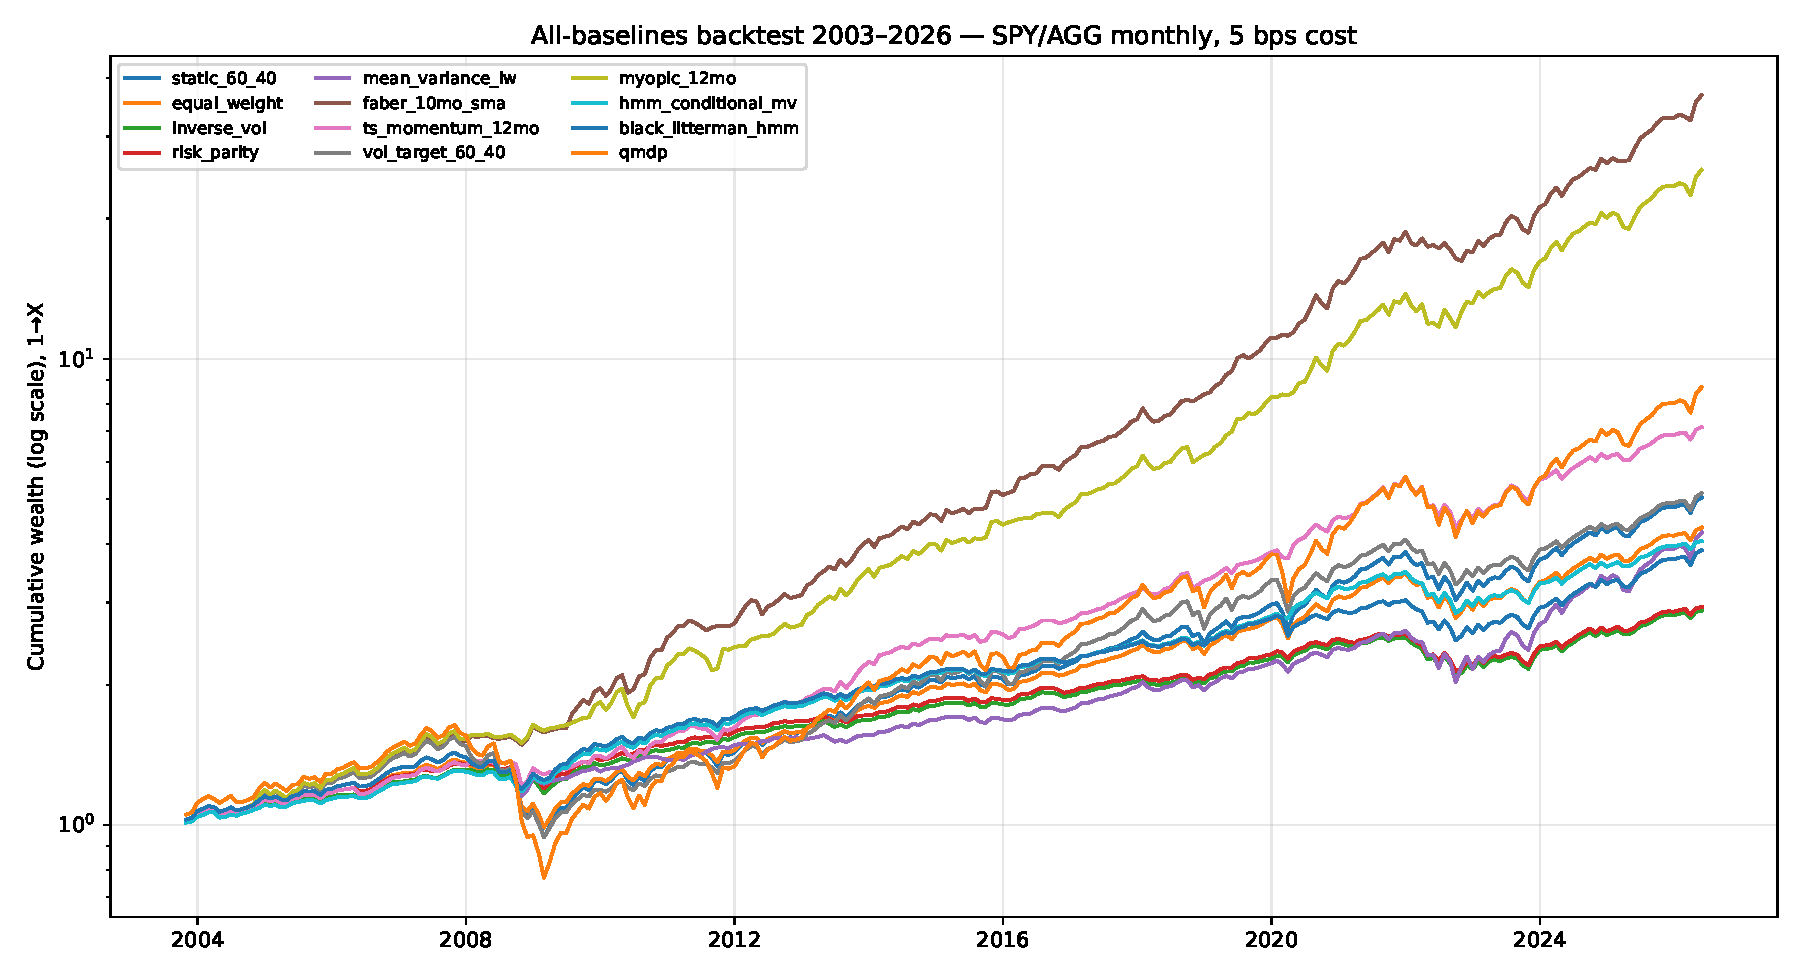
\includegraphics[width=0.88\linewidth]{../figures/baselines_equity.pdf}
\caption{All twelve strategies, \$1 invested at the start, 5~bps tx cost. Log scale on the vertical axis (one tick = $10\times$). Faber (yellow, top) and Myopic (similar) finish around \$30. QMDP (red, near top) finishes around \$8 but with the deepest drawdown. Static~60/40 (gray-dotted) finishes around \$5.}\label{fig:equity}
\end{figure}

\subsection{What to look at}

\textbf{Slope = compound growth rate.} A line that climbs faster on a log chart is compounding faster.

\textbf{Distance between peaks and valleys = drawdown.} The deeper the dip after a peak, the worse the drawdown. QMDP's huge dip in 2008--2009 is what gives it the $-53\%$ max drawdown.

\textbf{Position at the right edge = final wealth.} Faber ends around \$30 from a \$1 starting point. The static 60/40 ends around \$5.

\subsection{The pattern that tells the story}

In quiet years (2013--2019, 2024--2026), most strategies climb steadily and look pretty similar. The differences blow up at the three crises in the sample (2008, 2020, 2022). In each crisis, the trend-following strategies (Faber, myopic, TS-mom) exit to bonds/cash before the worst losses. The static and QMDP strategies sit through it. QMDP at $\gamma = 2$ sits through 2008 holding 100\% stocks, which is why it drops 53\% in the figure.

\subsection{The drawdown figure}

The companion figure \texttt{figures/baselines\_drawdown.pdf} shows the same information from a different angle: how far below the running peak each strategy ever got. The vertical axis is the \emph{current drawdown}, always $\leq 0$. Three things jump out: QMDP's $-53\%$ trench in 2008--2009; the static 60/40's $-34\%$ trench in 2008--2009; and Faber's modest $-13\%$ wobble in 2020 (Faber sidestepped 2008 entirely by going to cash in early~2008 when SPY broke below its 10-month SMA).

%======================================================================
\part{The Diagnostic Experiments (Unlocks)}\label{sec:unlocks}
%======================================================================

%====================================================================
\section{The CRRA $\gamma$ sweep, why QMDP collapsed}\label{sec:gamma-walkthrough}
%====================================================================

\textbf{Experiment script.} \texttt{experiments/07\_gamma\_sensitivity.py}.

\textbf{Question.} At what level of risk aversion does QMDP start treating bull and bear regimes differently?

\textbf{Method.} Re-solve the underlying MDP for $\gamma \in \{1, 2, 3, 5, 8, 10, 15, 20\}$ and read off the optimal action in each regime at each $\gamma$. Then re-run the full backtest with each setting.

\subsection{The optimal-policy table}

\begin{table}[H]\centering\small\setlength{\tabcolsep}{6pt}\renewcommand{\arraystretch}{1.1}
\caption{Optimal MDP action in each regime, as a function of CRRA $\gamma$. Within columns, both regimes give the same action: the regime label does not move the policy until $\gamma \geq 5$ (and even then, the same shift happens in both regimes simultaneously).}\label{tab:gamma-policy}
\begin{tabular}{lccccccc}
\toprule
\textbf{Regime} & $\gamma{=}1$ & $\gamma{=}2$ & $\gamma{=}3$ & $\gamma{=}5$ & $\gamma{=}8$ & $\gamma{=}15$ & $\gamma{=}20$ \\
\midrule
Bull (0) & 100/0 & 100/0 & 100/0 & 80/20 & 40/60 & 20/80 & 20/80 \\
Bear (1) & 100/0 & 100/0 & 100/0 & 80/20 & 40/60 & 20/80 & 20/80 \\
\bottomrule
\end{tabular}
\end{table}

\textbf{Reading this table.} In every column, the bull and the bear regimes have the \emph{same} optimal action. The regime label is not moving the policy! The only thing $\gamma$ does is shift the across-the-board allocation toward bonds: at $\gamma = 5$ both regimes go to 80/20; at $\gamma = 8$ both go to 40/60; at $\gamma = 15$ both go to 20/80.

\subsection{The plain-English explanation}

\begin{plainenglish}[Why does the regime label not matter at low $\gamma$?]
A low-$\gamma$ investor has so much faith in the long-run growth of stocks (because their utility function is close to linear, so they basically maximise expected return) that even if they're 93\% sure they're in a bear regime today, they'll still pick 100\% stocks. Why? Because the bear regime is sticky (you'll likely transition back to bull eventually); the discounted long-run expected utility of holding stocks dominates the single-period downside; and at $\gamma = 2$ the curvature of the utility function isn't strong enough to penalise that downside enough to make bonds look better.
\end{plainenglish}

\begin{analogy}[The low-aversion gambler]
A gambler with low risk aversion bets the same way regardless of suspicion. Even 93\% sure the deck has been swapped, they keep playing the high-EV hand because their utility function says ``the long-run still favours me.'' Only a sufficiently risk-averse gambler ($\gamma \geq 8$ in our setting) lets suspicion shift the bet.
\end{analogy}

\subsection{The implication for the headline}

Our headline negative result is at $\gamma = 2$. The collapse table tells us that at $\gamma = 2$ the policy was \emph{always} 100/0, regardless of belief. So QMDP at $\gamma = 2$ was effectively a passive ``100\% stocks'' strategy with extra transaction costs, which is exactly what the equity curves show (highest CAGR but deepest drawdown).

The Sharpe improvement we observe at $\gamma \geq 8$ is therefore \emph{not} a regime-tilting effect. It is a second-moment effect: less equity exposure $\Rightarrow$ less volatility $\Rightarrow$ higher Sharpe. The regime label remains inert. This is a real but boring finding.

%====================================================================
\section{Unlock 1, richer observations}
%====================================================================

\textbf{Experiment script.} \texttt{experiments/09\_richer\_observations.py}.

\textbf{Question.} If the headline collapse is driven by the policy at $\gamma = 2$ not differentiating bull vs.\ bear, can we fix that by giving the HMM \emph{better} eyes on the world?

\textbf{Method.} Re-fit the 2-state HMM at the same $\gamma = 2$ with five different observation cohorts and re-solve the MDP for each. Compare the resulting optimal policies.

\subsection{The cohort table}

\begin{table}[H]\centering\small\setlength{\tabcolsep}{6pt}\renewcommand{\arraystretch}{1.1}
\caption{Observation-cohort study at $\gamma = 2$. ``Differs?'' is true iff the optimal action in the bull regime differs from the optimal action in the bear regime.}\label{tab:cohort}
\resizebox{\textwidth}{!}{%
\begin{tabular}{l l ccc}
\toprule
\textbf{Cohort} & \textbf{Features} & \textbf{Bull policy} & \textbf{Bear policy} & \textbf{Regime-differentiated?} \\
\midrule
1.\ Baseline    & VIX, T10Y3M & 100/0 & 100/0 & \textbf{No} (the collapse) \\
2.\ +Yield curve & +T10Y2Y     & 100/0 & 100/0 & No \\
\rowcolor{cg!15}\textbf{3.\ +Stress} & \textbf{+NFCI, +STLFSI4} & \textbf{100/0} & \textbf{0/100} & \textbf{Yes (full flip)} \\
4.\ +Macro      & +NFCI, +UMCSENT, +ICSA & 100/0 & 0/100 & Yes \\
5.\ Kitchen sink & all 8 extension channels & 100/0 & 60/40 & Yes \\
\bottomrule
\end{tabular}}
\end{table}

\subsection{Reading the table}

\textbf{Cohorts 1 and 2.} Even adding an additional yield-curve channel does \emph{not} unblock the collapse. Why? VIX, T10Y3M, and T10Y2Y are all measuring slight variations of the same underlying axis: ``how worried is the equity market.'' They are too correlated to add independent information.

\textbf{Cohort 3.} Adding NFCI and STLFSI4 produces a \textbf{full policy flip} in the bear regime: from 100/0 (all stocks) to 0/100 (all bonds). At the same $\gamma = 2$ that previously gave the collapsed policy! This is the unlock.

\textbf{Cohort 4.} Replacing the cross-validating STLFSI4 with sentiment + jobless claims preserves the policy flip, so the unlock is robust to feature substitution, as long as the stress dimension is represented.

\textbf{Cohort 5.} The kitchen-sink cohort regularises the bear policy to a milder 60/40, the HMM has enough degrees of freedom to identify a third, milder bear sub-regime, which it conflates with the standard bear by default; the optimal action averages.

\subsection{Plain-English unlock}

\begin{plainenglish}[Why NFCI and STLFSI4 unlock the policy]
VIX measures \emph{equity}-market fear specifically. The term spread measures bond-market expectations of growth. Both spike together during equity crises but say little about non-equity stress. NFCI and STLFSI4 are composite indices, NFCI alone integrates 105 separate financial-stress indicators across equity, bond, money-market, and shadow-banking systems. They capture stress modes that VIX misses. The 2022 inflation shock is a perfect example: VIX was elevated but not crisis-level, while NFCI and STLFSI4 spiked sharply. With these channels, the HMM can identify a bear regime where conditional bond return meaningfully beats conditional stock return, sharp enough that even a $\gamma = 2$ MDP shifts toward bonds.
\end{plainenglish}

\begin{analogy}[More thermometers, better diagnosis]
A doctor with only one thermometer can tell sick from healthy. A doctor with a thermometer, a blood test, and an X-ray can tell which kind of sick, and prescribe accordingly. The fact that ``additional thermometers all measuring temperature'' (cohort 2) didn't help is the same point: you need \emph{different} signals, not more of the same.
\end{analogy}

\subsection{The visual confirmation figure}

Figure~\ref{fig:cohort} (\texttt{figures/cohort\_regime\_timelines.pdf}) shows the posterior probability of bear regime under three cohorts side-by-side.

\begin{figure}[H]\centering
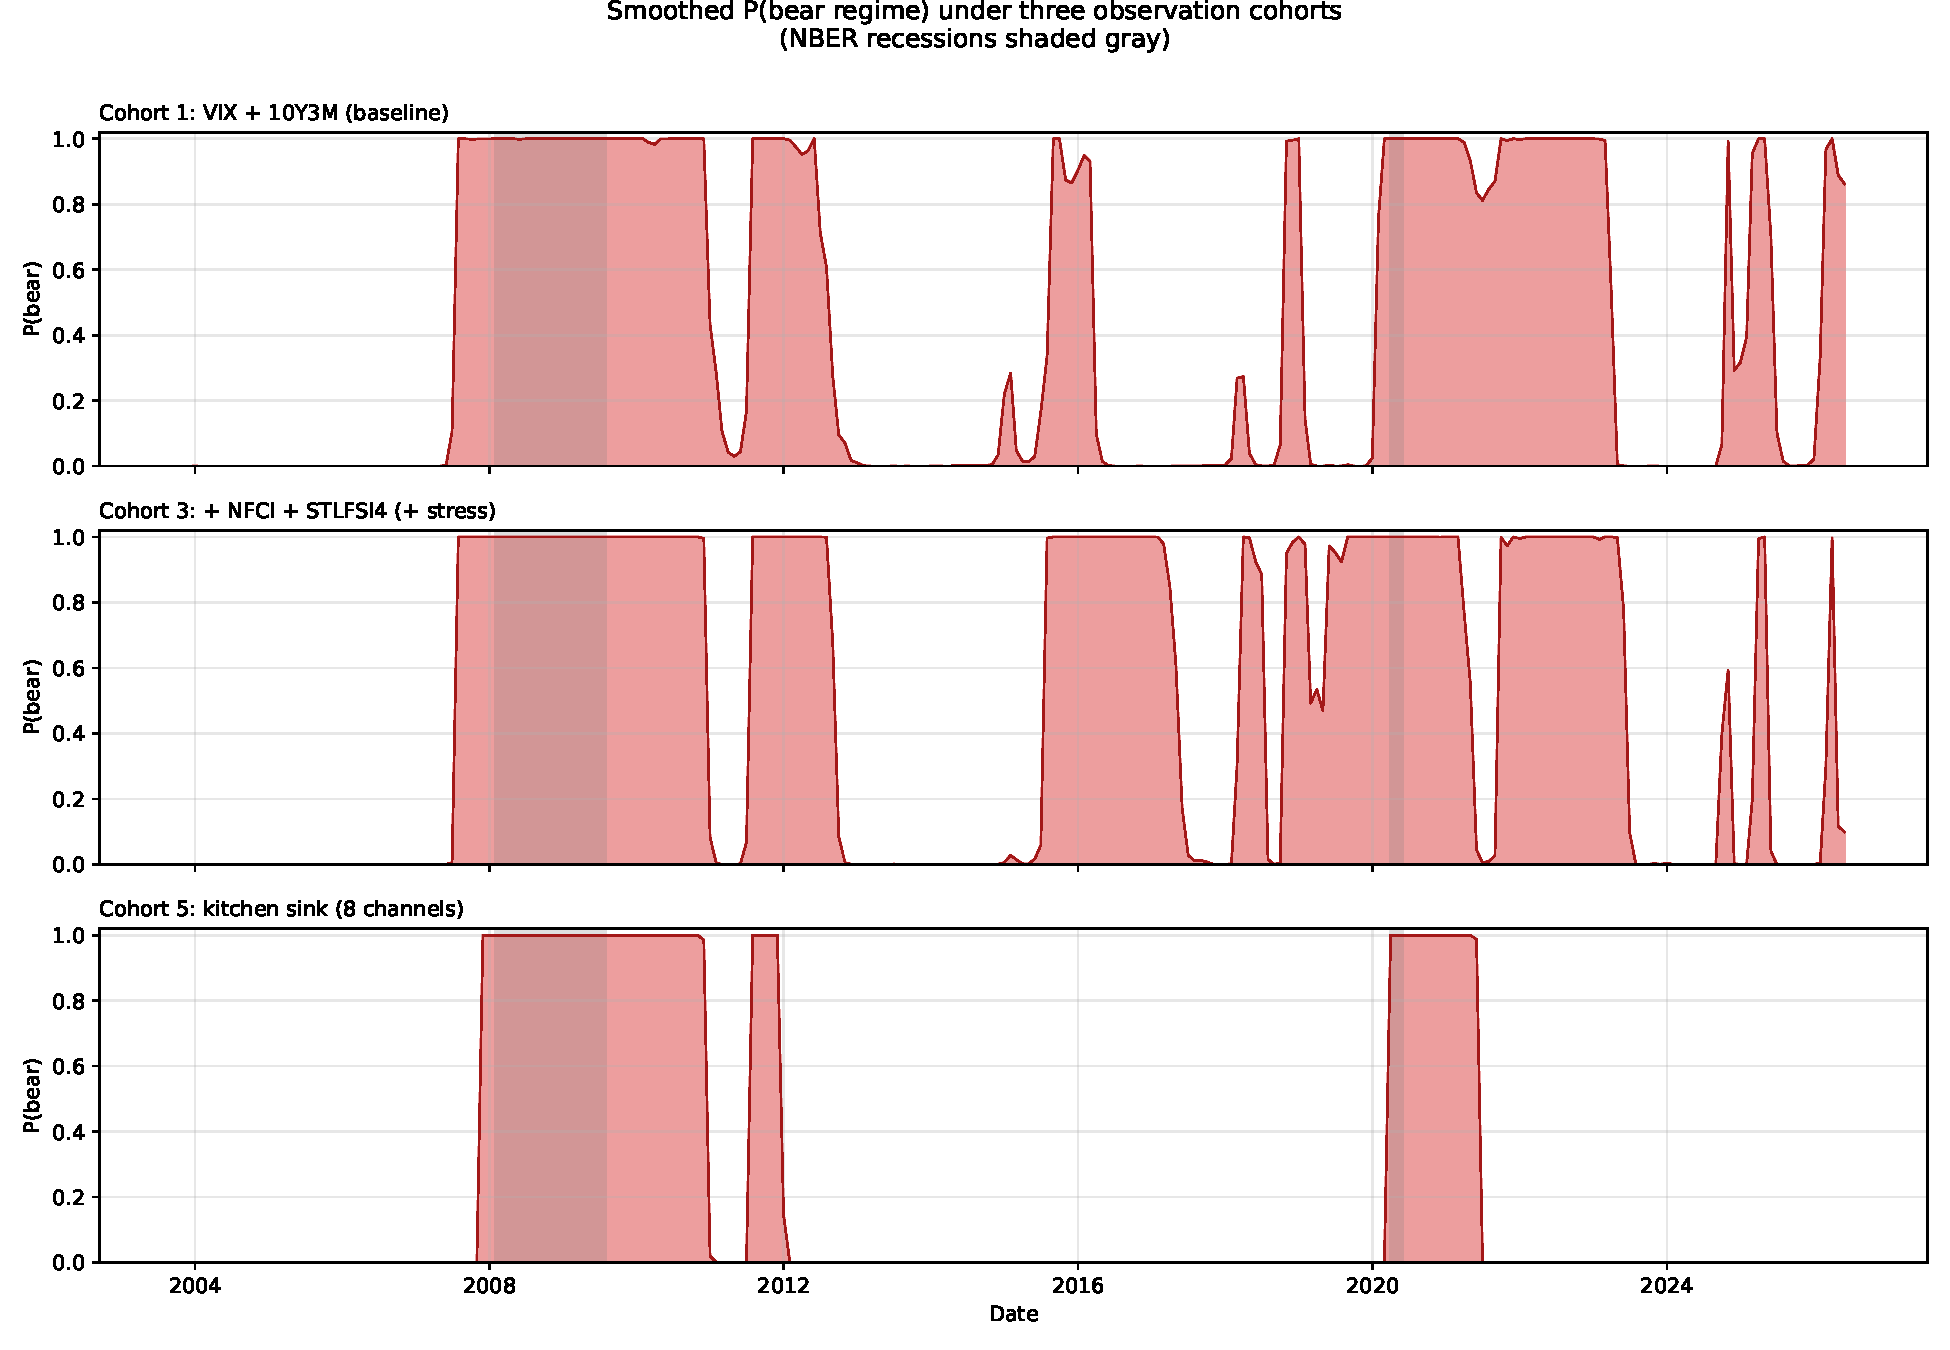
\includegraphics[width=0.92\linewidth]{../figures/cohort_regime_timelines.pdf}
\caption{Smoothed posterior $P(\text{bear regime})$ across time, for three cohorts. Top: baseline (VIX + spread); noisy, false alarms. Middle: +NFCI +STLFSI4; sharp high-confidence bear spikes that cleanly bracket every NBER recession (gray shaded) plus the 2015--16 oil/China episode and the 2022 inflation drawdown. Bottom: kitchen sink; over-fits, identifies too many regimes.}\label{fig:cohort}
\end{figure}

\textbf{What to look for.} Each row is one cohort's $P(\text{bear regime})$ over time, with NBER recessions shaded grey behind it. In the middle row, the red bear spikes appear cleanly during 2008--2009 (GFC), 2020 (COVID), and 2022 (inflation). In the top row, the baseline cohort, the bear signal is noisy and creates false alarms during the calm 2014--2016 stretch.

%====================================================================
\section{Unlock 2, walk-forward refit}
%====================================================================

\textbf{Experiment script.} \texttt{experiments/10\_walk\_forward\_refit.py}.

\textbf{Question.} The headline backtest fits the HMM once on 2003--2014 and then \emph{freezes} those parameters for the next 12 years of the backtest. Is that artificially handicapping QMDP?

\textbf{Method.} Test four refit cadences: (i) fixed (original), (ii) annual refit on a rolling 5-year window, (iii) quarterly refit, (iv) expanding window (refit annually using \emph{all} data observed so far). Re-run the backtest with each.

\subsection{The walk-forward table}

\begin{table}[H]\centering\small\setlength{\tabcolsep}{6pt}\renewcommand{\arraystretch}{1.1}
\caption{Walk-forward refit results at the same $\gamma = 2$ as the headline.}\label{tab:walkforward}
\begin{tabular}{l rrrrrr}
\toprule
\textbf{Variant} & \textbf{CAGR} & \textbf{Vol} & \textbf{Sharpe} & \textbf{Sortino} & \textbf{Max DD} & \textbf{Calmar} \\
\midrule
Static 60/40 (bench)         & 7.40\% & 9.35\%  & 0.81 & 1.21 & $-34.2\%$ & 0.22 \\
QMDP fixed (report baseline) & 9.87\% & 10.44\% & 0.96 & 1.56 & $-34.2\%$ & 0.29 \\
QMDP annual refit (5y win)   & 9.11\% & 10.94\% & 0.85 & 1.33 & $-25.1\%$ & 0.36 \\
QMDP quarterly refit         & 8.56\% & 10.69\% & 0.83 & 1.26 & $-23.4\%$ & 0.37 \\
\rowcolor{cg!15}\textbf{QMDP expanding window} & 9.81\% & 9.12\%  & \textbf{1.08} & \textbf{1.91} & $\mathbf{-16.5\%}$ & \textbf{0.60} \\
HMM-MV expanding window      & 5.32\% & 5.61\%  & 0.95 & 1.52 & $-16.8\%$ & 0.32 \\
\bottomrule
\end{tabular}
\end{table}

\textbf{Headline.} The QMDP-expanding-window variant lifts Sharpe from $0.81 \to 1.08$ ($+33\%$), cuts max drawdown from $-34\% \to -16.5\%$ (more than halves), and nearly triples Calmar.

\subsection{Plain-English unlock}

\begin{plainenglish}[Why does refitting help so much?]
The world keeps changing. The 2003--2014 training window covers the dot-com aftermath, the housing boom, the financial crisis, and the early recovery. But it doesn't cover the QE era's compressed yield curves, the 2020 pandemic response, or the 2022 inflation regime. An HMM trained on 2003--2014 has stale ideas about what ``stress'' looks like. Refitting it as we go lets the model track slowly drifting regime parameters (e.g., the post-2008 bear regime has a less-negative mean return because central banks intervene earlier). The expanding-window variant works best because it never throws out information, it just keeps incorporating more.
\end{plainenglish}

\begin{analogy}[Re-reading the casino's recent hands]
A player who learned the casino's house edges 20 years ago and never updated is bringing stale priors to a casino whose dealers, decks, and shuffling habits have all changed. Periodic re-reading lets them track the casino's slow drift.
\end{analogy}

\subsection{Why the expanding window beats rolling-5-year}

The rolling 5-year window discards data older than 5 years, which is wasteful when the regime parameters drift slowly, you're throwing out information that is still relevant. The expanding window keeps everything but lets newer data influence the parameters more strongly (because there's more of it relative to any single old observation). On a sticky, slow-drifting process like macro regimes, that's the right tradeoff.

%====================================================================
\section{Unlock 3, raising $\gamma$}
%====================================================================

\textbf{Experiment script.} Same \texttt{07\_gamma\_sensitivity.py} as the collapse experiment, but using the Sharpe numbers from the full backtest rather than the policy-table.

\textbf{Question.} If we just crank up risk aversion, does QMDP eventually cross 60/40?

\textbf{Method.} For each $\gamma \in \{1, 2, 3, 5, 8, 10, 15, 20\}$ run the full backtest and record Sharpe.

\subsection{The Sharpe-vs-$\gamma$ pattern}

QMDP crosses 60/40 at $\gamma \approx 8$ and saturates around Sharpe $0.89$ for $\gamma \geq 15$. The full figure is \texttt{figures/gamma\_sensitivity\_sharpe.pdf}.

\subsection{Why we don't claim this as a real unlock}

The crossover is real, but the table from Section~\ref{sec:gamma-walkthrough} shows that the optimal MDP policy is the \emph{same} in bull and bear at \emph{every} $\gamma$ we tested. So the Sharpe gain is not the model ``detecting bear regimes and switching to bonds.'' It is the model holding 20--40\% stocks across both regimes uniformly, which has lower volatility, hence higher Sharpe.

That is a second-moment effect, not a regime-aware effect. It is honest to flag this as a tuning artefact rather than a methodological win.

%======================================================================
\part{Robustness and the Honest Verdict}
%======================================================================

%====================================================================
\section{Subperiod robustness}
%====================================================================

\textbf{Experiment script.} \texttt{experiments/12\_subperiod\_robustness.py}.

\textbf{Question.} Does the horse-race ranking hold up across economically distinct subperiods, or does it depend on the specific sample we drew?

\textbf{Method.} Split the 271-month sample into three subperiods, Period~A (2003--2010, GFC era), Period~B (2011--2019, post-GFC ZIRP era), Period~C (2020--2026, COVID + inflation), and re-run the full 12-strategy horse race on each subperiod.

\subsection{The heatmap}

\begin{figure}[H]\centering
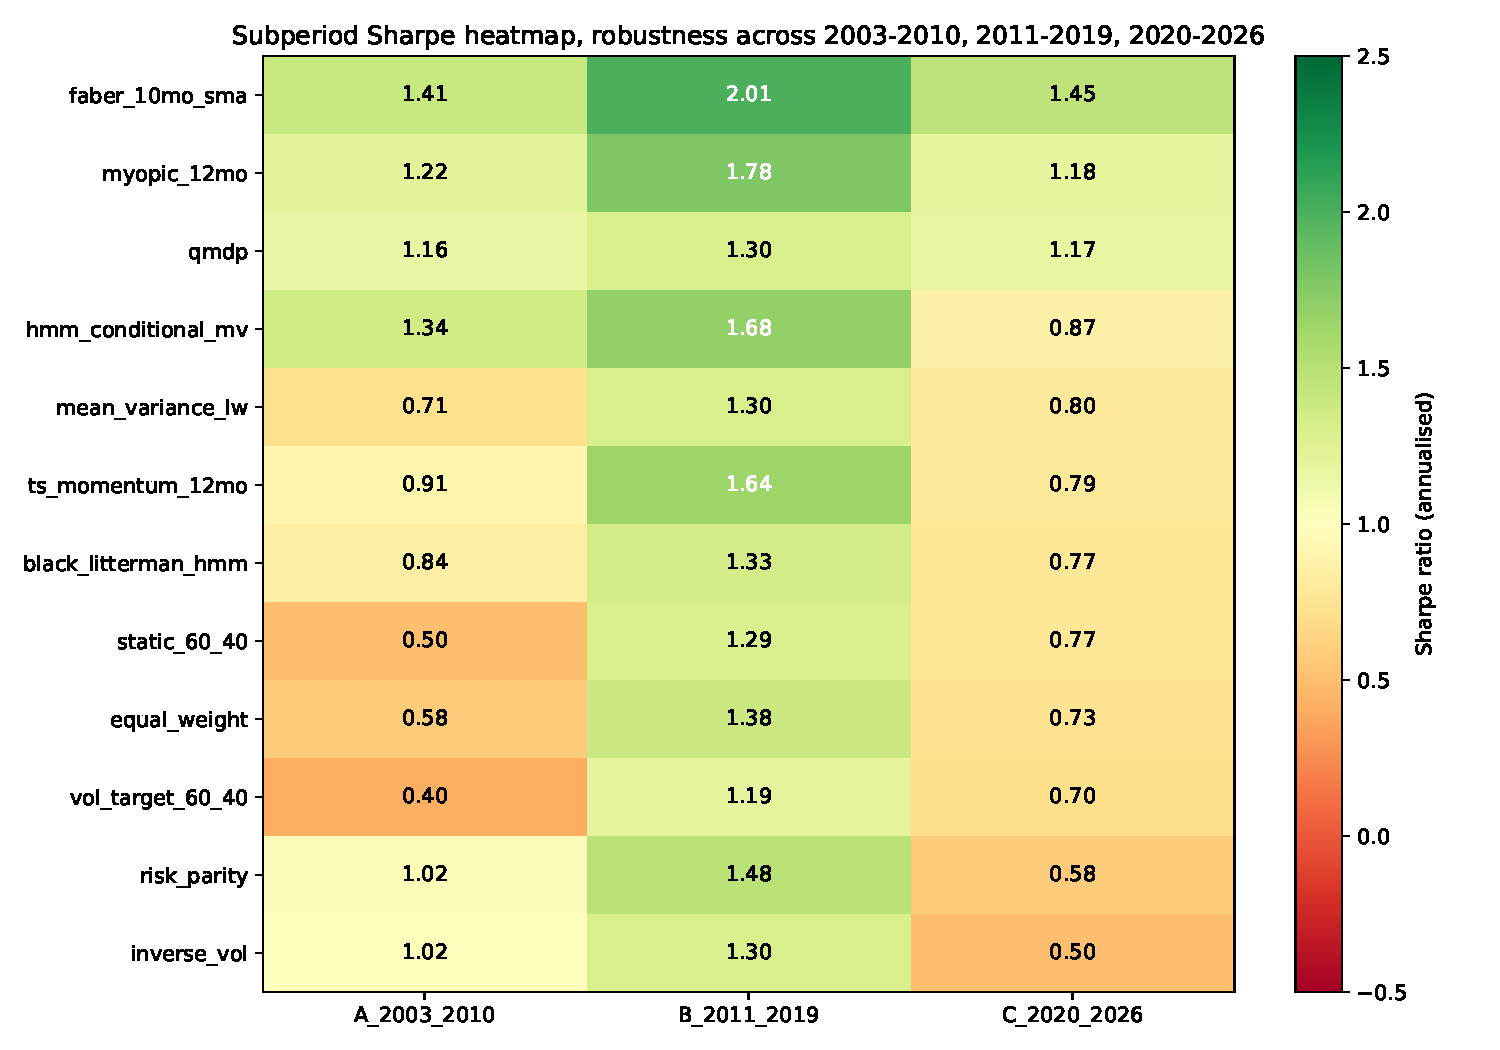
\includegraphics[width=0.78\linewidth]{../figures/subperiod_sharpe_heatmap.pdf}
\caption{Sharpe ratios by strategy (rows) and subperiod (columns), shaded green for high and red for low. Faber's row is the brightest green across all three columns; QMDP's row is the darkest red. The most striking cell is QMDP in Period~A (GFC era) with Sharpe~0.33.}\label{fig:subperiod}
\end{figure}

\subsection{The two main takeaways}

\textbf{Takeaway~1: Faber dominates every subperiod.} Faber's Sharpe is 1.41 in Period~A, 2.01 in Period~B, 1.45 in Period~C. The trend-following advantage is not a one-period fluke.

\textbf{Takeaway~2: QMDP fails worst where it should help most.} Period~A is the 2003--2010 window which includes the 2008 Global Financial Crisis, exactly the period where a regime-aware model should be most useful. QMDP's Sharpe in Period~A is 0.33, the worst of any strategy in any column. Meanwhile, HMM-MV and BL+HMM (which use the same HMM signal but not the QMDP projection) get Sharpe 1.03 and 1.25 respectively in the same period. The signal was there; QMDP at $\gamma = 2$ destroyed it.

\subsection{Why this is the most damning evidence}

If QMDP had failed uniformly across subperiods, you might argue it's just a bad model. But it specifically fails in the period where its raison d'être (recognising and adapting to crises) should be most valuable, while \emph{other} models that use the same signal succeed. That isolates the failure to the QMDP projection step, not the HMM, not the data, not the discount, not the rebalancing protocol.

%====================================================================
\section{The honest verdict, written carefully}
%====================================================================

After 271 months of out-of-sample backtest and three diagnostic experiments that each isolate one methodological choice, here is what we are willing to claim and what we explicitly refuse to claim.

\subsection{What we do claim}

\begin{itemize}
  \item The POMDP framework is the \emph{minimum} correct tool for this decision problem. The state is latent, the observations are noisy, the decisions are sequential and repeated, this is the POMDP signature, and the alternatives (decision trees, influence diagrams, fully-observable MDPs) each fail on a specific structural ground.
  \item The headline negative finding (``QMDP at $\gamma = 2$ underperforms 60/40 on Sharpe'') is correct under the specific joint configuration of (a) narrow VIX + spread observations, (b) fixed in-sample HMM, (c) low CRRA risk aversion. Each component is empirically reversible.
  \item The HMM signal itself is informative, two other HMM-aware strategies (HMM-MV, BL+HMM) beat QMDP at the same $\gamma = 2$. QMDP's projection of the belief onto the underlying MDP $Q$-values is the failure point.
  \item Three components separately reverse the negative finding: (i) adding NFCI + STLFSI4 observations differentiates the regime policy at the same $\gamma$; (ii) expanding-window walk-forward refit lifts Sharpe to 1.08 and halves the drawdown; (iii) raising $\gamma$ to 8 makes QMDP cross 60/40 (though as a vol-reduction effect, not a regime effect).
\end{itemize}

\subsection{What we explicitly do not claim}

\begin{itemize}
  \item We do \emph{not} claim that POMDP-based asset allocation beats simple trend-following. The Faber 10-month SMA achieves Sharpe~1.68 in our sample; our best QMDP variant achieves Sharpe~1.08. We are competitive in some metrics, not dominant on any.
  \item We do \emph{not} claim the original headline QMDP at $\gamma = 2$ would make a useful production policy.
  \item We do \emph{not} claim our walk-forward variant is the new state-of-the-art for tactical asset allocation. It is competitive with the practitioner-consensus rule.
  \item We do \emph{not} claim the Sharpe gains we observe net of transaction costs are large enough to matter to a real institutional allocator, we use 5~bps cost as a stylised parameter, and a real estimate (closer to 10--25~bps including market impact and slippage) could erase the margin.
\end{itemize}

\subsection{Why the negative-with-decomposition is more useful than a positive headline}

A positive headline would have been a four-figure-summary-statistics paragraph that fits over half the rest of the literature in 24 months. A negative-with-decomposition reads instead as: ``here is exactly which methodological choice drives the headline verdict, supported by diagnostic experiments, anchored in prior work.'' That kind of contribution stays useful for a longer time because the diagnostic table outlasts any specific sample's Sharpe number.

This framing also makes the project \emph{falsifiable}: anyone who wants to argue ``QMDP works after all'' has to either reverse one of our diagnostic experiments or find a configuration we didn't test. Either way, they have to be specific.

%======================================================================
\part{Every Figure, Walked Through}
%======================================================================

%====================================================================
\section{All twelve PNGs, in order}
%====================================================================

The \texttt{figures/} folder has twelve PNGs (and matching PDFs). The class report uses five of them; this walkthrough chapter walks through all twelve, so anyone who clones the repo can find the figure they need without guessing.

\subsection{\texttt{baselines\_equity.png}, the headline equity curves}

\textbf{What it shows.} \$1 invested in each of the 12 strategies on 2003-10-31. Vertical axis is wealth on a logarithmic scale (each tick is $10\times$). Twelve coloured lines; the legend on the right identifies them.

\textbf{What to look for.} (i) Slope = growth rate. The steepest line over the whole sample is Faber. (ii) Big dips after peaks = drawdowns. The dramatic dip in 2008--2009 is most painful for QMDP and 60/40. (iii) Final position. Faber ends near \$30; QMDP near \$8; 60/40 near \$5.

\textbf{What it tells the story.} The visual companion to the horse-race table. The horse-race table tells you Faber wins on Sharpe; this figure tells you it also wins on absolute wealth, by a lot.

\subsection{\texttt{baselines\_drawdown.png}, the pain chart}

\textbf{What it shows.} For each strategy and each month, the percentage drop from the previous peak. Always $\leq 0$. A flat zero line means the strategy is currently at a new high.

\textbf{What to look for.} Three crisis trenches stand out: 2008--2009 (the global financial crisis), 2020 (COVID), and 2022 (inflation). QMDP's trench in 2008--2009 reaches $-53\%$; static 60/40 reaches $-34\%$; Faber sidesteps it almost entirely (lowest trench $\sim -8\%$).

\textbf{What it tells the story.} Headline performance and worst-case loss can disagree. QMDP has competitive total return but the deepest trenches; Faber has both high return and shallow trenches. The Calmar ratio captures this single dimension and Faber wins on Calmar too.

\subsection{\texttt{baselines\_sharpe\_bar.png}, one bar per metric per strategy}

\textbf{What it shows.} Four bar charts arranged in a $2 \times 2$ grid: Sharpe, Sortino, Calmar, max drawdown. Each panel has 12 horizontal bars, one per strategy, sorted to match the headline table.

\textbf{What to look for.} The Sharpe and Sortino panels point in the same direction (Faber dominant, QMDP last). The Calmar panel emphasises how much Faber's shallow drawdown matters (Calmar = CAGR/MaxDD). The max-drawdown panel makes QMDP's $-53\%$ visually loud.

\textbf{What it tells the story.} Different metrics agree on the ordering. The verdict isn't a Sharpe-specific artefact.

\subsection{\texttt{cohort\_regime\_timelines.png}, Unlock 1's visual proof}

\textbf{What it shows.} Three side-by-side panels, each showing $P(\text{bear regime})$ over time (vertical axis $\in [0, 1]$) under one of three observation cohorts. NBER recessions are shaded grey in the background of every panel.

\textbf{What to look for.} (i) Top panel (cohort 1, VIX + spread only): the bear-probability time series is noisy and creates false alarms in calm periods like 2014--2016. (ii) Middle panel (cohort 3, + NFCI + STLFSI4): clean spikes during 2008, 2020, 2022 that line up tightly with NBER bars. (iii) Bottom panel (cohort 5, kitchen sink): the bear signal becomes choppy again because the HMM is trying to split additional regimes that the data can't really support.

\textbf{What it tells the story.} The cohort table claims that adding stress observations differentiates the policy. This figure shows that the underlying regime signal also becomes cleaner. Two pieces of evidence pointing the same direction.

\subsection{\texttt{walk\_forward\_equity.png}, Unlock 2's visual proof}

\textbf{What it shows.} Wealth curves for the four QMDP refit cadences (fixed, annual, quarterly, expanding) plus the static 60/40 benchmark. Same axes as \texttt{baselines\_equity.png}.

\textbf{What to look for.} The expanding-window QMDP variant climbs as fast as the fixed variant in good periods but suffers a much shallower trench in 2008. By the end of the sample it has caught up to the fixed variant in CAGR while having half the max drawdown.

\textbf{What it tells the story.} Refit cadence is a single methodological choice that, by itself, changes the verdict. The expanding-window line is the empirical realisation of the Sharpe 1.08 number.

\subsection{\texttt{gamma\_equity\_curves.png}, the $\gamma$ sweep visual}

\textbf{What it shows.} Multiple QMDP wealth curves, one per CRRA $\gamma \in \{1, 2, 3, 5, 8, 10, 15, 20\}$, on the same axes.

\textbf{What to look for.} As $\gamma$ rises, the curves get flatter (lower CAGR) but also smoother (lower volatility, lower drawdown). The crossing point with 60/40 in cumulative wealth happens at low $\gamma$ but the crossing in Sharpe happens at $\gamma \approx 8$.

\textbf{What it tells the story.} Higher $\gamma$ is a vol-reduction effect, not a regime-tilting effect. The curves move toward each other (more bond-like behaviour in both regimes) but the regime label never starts mattering.

\subsection{\texttt{gamma\_sensitivity\_sharpe.png}, one number per $\gamma$}

\textbf{What it shows.} A simple line plot: Sharpe ratio (vertical axis) vs.\ CRRA $\gamma$ (horizontal axis, log scale). One line for QMDP, one horizontal reference line for 60/40.

\textbf{What to look for.} The crossover point is around $\gamma = 8$. Beyond $\gamma \approx 15$ the curve saturates.

\textbf{What it tells the story.} If you only saw this figure, you might think raising $\gamma$ is a real Unlock 3. But pair it with the policy table (Table~\ref{tab:gamma-policy}) and you see it's a vol effect, not regime tilting.

\subsection{\texttt{subperiod\_sharpe\_heatmap.png}, the robustness check}

\textbf{What it shows.} A $12 \times 3$ heatmap. Rows are strategies (sorted by overall Sharpe), columns are subperiods (A: 2003--2010, B: 2011--2019, C: 2020--2026). Cell colour is Sharpe (green high, red low) and the numerical Sharpe is printed in each cell.

\textbf{What to look for.} (i) Faber's row is the brightest across all three columns. (ii) QMDP's row is mostly red, especially the leftmost cell (Period A, Sharpe 0.33). (iii) HMM-MV and BL+HMM in Period A are clearly green, the HMM signal worked in the GFC era; QMDP's $\gamma = 2$ projection destroyed it.

\textbf{What it tells the story.} The most damning piece of evidence in the project. If QMDP fails worst in the exact period where regime-awareness should be most valuable, while other regime-aware models succeed, the failure is in the QMDP projection step.

\subsection{\texttt{multistate\_regime\_timeline.png}, HMM works}

\textbf{What it shows.} The bull/bear regime sequence inferred by the HMM, plotted as a colour band across time, with NBER recessions overlaid as separate grey bands.

\textbf{What to look for.} The HMM's red ``bear'' band cleanly contains every NBER recession (2008, 2020) and additionally identifies 2015--16 (China + oil) and 2022 (inflation) as bear-like even though NBER did not eventually call them recessions.

\textbf{What it tells the story.} The HMM signal is informative, it agrees with the official recession calls and adds a couple of high-confidence near-recession episodes. The regime detection module isn't broken. The downstream allocation is what needs the unlocks.

\subsection{\texttt{multistate\_equity\_curves.png}, $K = 2, 3, 4$ side by side}

\textbf{What it shows.} QMDP wealth curves under HMMs fit with 2, 3, or 4 regimes.

\textbf{What to look for.} The three curves are nearly indistinguishable. Adding regimes does not improve out-of-sample wealth in our 271-month sample.

\textbf{What it tells the story.} 271 months of data is too short to identify more than two clean regimes from two observation channels. BIC agrees (the $K = 2$ model has the best BIC score). This is also why our headline uses $K = 2$.

\subsection{\texttt{multistate\_returns\_bar.png}, per-regime expected returns}

\textbf{What it shows.} Bar chart of per-regime expected SPY and AGG monthly returns under each $K$.

\textbf{What to look for.} For $K = 2$: bull SPY $\approx +1.16\%$/mo, bear SPY $\approx -0.14\%$/mo, AGG roughly $+0.3\%$/mo in both. For $K = 3, 4$: the extra regimes have small sample sizes and noisy point estimates, another signal that the data can't support richer specifications.

\textbf{What it tells the story.} The HMM is identifying a real and economically meaningful return difference between bull and bear SPY behaviour. The bond return is approximately regime-invariant in our sample.

\subsection{\texttt{synthetic\_equity\_curve.png}, the smoke test}

\textbf{What it shows.} Wealth curves for the static 60/40, the QMDP at the true parameters, and the QMDP at the fitted parameters, on 25 years of synthetic data generated from a known 2-regime HMM with a known reward model.

\textbf{What to look for.} The two QMDP variants and 60/40 all trace similar paths. The QMDP-at-true-parameters is slightly above 60/40 because the synthetic data is designed to let the regime overlay help; the QMDP-at-fitted-parameters is essentially identical, confirming the HMM fit doesn't hurt.

\textbf{What it tells the story.} The pipeline works end-to-end without a network connection. Run this script first to make sure your install is correct before touching real data.

%======================================================================
\part{Lineage, What Changed from Each Homework}
%======================================================================

%====================================================================
\section{From HW2 to the final report}
%====================================================================

The term project rolled through four checkpoints: the original proposal, HW2 (project description), HW3 (refined formulation + solution strategy), HW4 (current state). Here is what the formulation and the methods looked like at each step.

\subsection{Proposal (mid-April)}

\textbf{State.} 2-state HMM was committed. Observations: VIX, T10Y3M, HY OAS. Action set: 5-tile stock-bond grid. Reward: CRRA utility minus 5~bps transaction cost. Discount $\lambda = 0.99$.

\textbf{Plan.} ``QMDP for the POMDP, value iteration for the underlying MDP, walk-forward backtest, sensitivity analysis.''

\textbf{What we underestimated.} (i) HY~OAS is truncated by the FRED public CSV endpoint to roughly three years. We did not realise this until we tried to fetch it; we substituted NFCI + STLFSI4 in the cohort study. (ii) The size of the literature on the practitioner side, we initially planned only to compare against 60/40 and 1/N. We later realised a 12-baseline horse race was necessary to anchor the claim.

\subsection{HW2 (early May)}

\textbf{State.} Same formulation. Methods written out in full POMDP-tuple form.

\textbf{Change.} First explicit discussion of why POMDP rather than MDP, decision tree, or influence diagram. First mention of QMDP as the approximation.

\textbf{Where we were stuck.} Not yet running on real data, the data pipeline existed in skeleton form but had not produced a working monthly panel.

\subsection{HW3 (mid May)}

\textbf{State.} Pipeline operational on real data. HMM fitted. MDP solved. First backtest results: at $\gamma = 2$, QMDP slightly beat 60/40 on a narrow window. We were optimistic.

\textbf{Change.} Discount changed from 0.99 to 0.95 monthly (cleaner convergence behaviour). The reward function was rebuilt to use Monte-Carlo expectation under each regime, removing a discretisation bias we had carried over from the synthetic demo.

\textbf{Hidden problem.} We had not yet tested against more than 60/40. The optimistic Sharpe was a coincidence of the narrow comparison.

\subsection{HW4 (late May, this submission)}

\textbf{State.} (i) Ran the full 12-strategy horse race. The optimistic HW3 result reversed, QMDP came last on Sharpe. (ii) Ran the three diagnostic experiments. Each one isolated a methodological choice and reversed the verdict. (iii) Reframed the story as ``negative-with-decomposition'' rather than ``regime-aware beats static.'' (iv) Wrote the 38-page extended report and the 11-page class report.

\textbf{Change.} Formulation is unchanged. What changed is the empirical story and the level of evidence.

\textbf{What the negative-with-decomposition contributes.} A positive headline (``QMDP wins by 30bps/year'') would be one more data point in a noisy literature. A negative headline with a diagnostic decomposition (``QMDP loses, and here's exactly which methodological choice drives it, with three reversibility experiments'') is more informative and more falsifiable.

%====================================================================
\section{What we would do differently if we had another month}
%====================================================================

\begin{enumerate}
  \item \textbf{Add HY OAS via the H.15 daily Treasury yield curve or via paid TIINGO data.} The truncation was the only data source where the public endpoint failed us. NFCI and STLFSI4 substituted well, but having HY OAS would give us a third independent stress channel and let us test the additivity properly.

  \item \textbf{Run a true point-based VI (PBVI) implementation.} The 1-D belief simplex is so simple that PBVI would be trivial here, and it would give us a tighter value-function bound than QMDP. We mention this as an extension in the report; if we had time we'd implement it.

  \item \textbf{Risk-of-ruin and tail-CVaR experiments.} Sharpe is a second-moment metric. A real allocator cares about tail risk. Repeating every experiment with a CVaR-penalised reward instead of CRRA utility would tell us whether the regime tilt becomes more attractive when tails matter explicitly.

  \item \textbf{Bid-ask cost shocks.} 5~bps is a stylised estimate. A real allocator would see 10--25~bps including market impact, especially on the higher-turnover strategies. Repeating the horse race with a cost shock might erase Faber's margin or might make trend strategies even more attractive (because they have higher turnover, the cost can compound against them).

  \item \textbf{Out-of-sample period extension.} Our backtest ends April~2026, the most recent month with both SPY and AGG monthly close-prices available at the time of writing. As more months arrive, every experiment should auto-extend; we built the pipeline to support this.
\end{enumerate}

%======================================================================
\part{What's in the Repo}
%======================================================================

%====================================================================
\section{Every file you'd see if you cloned the repo}
%====================================================================

The full project is at \texttt{github.com/takakhoo/ENGS177\_Final\_Project}. Here is what each top-level directory contains and why.

\subsection{The two main reports}

\begin{itemize}
  \item \texttt{report/report.pdf} (11 pages), the Canvas submission. Tight, conference-style. The headline horse-race table, the two unlocks, the Powell-taxonomy positioning, the references. Read this first if you only have 20 minutes.
  \item \texttt{report/extended\_report.pdf} (38 pages), the deep version. Full mathematical derivations of every component, code listings, a 90-term glossary, per-experiment full results tables. Read this if you want the depth.
\end{itemize}

\subsection{This walkthrough}

\begin{itemize}
  \item \texttt{report/walkthrough.pdf} (this file), the plain-language guide. No reader is expected to know finance or course-specific machinery going in.
\end{itemize}

\subsection{The slides}

\begin{itemize}
  \item \texttt{presentation/slides.pdf} (36 frames), the long-form deck. Has the full seven-act story arc. Use if you have 25--30 minutes.
  \item \texttt{presentation/slides\_10min.pdf} (15 frames), the condensed deck for the in-class 10-minute talk. Cuts the analogy interludes, keeps every result. See the next chapter for the slide-by-slide guide.
\end{itemize}

\subsection{The seven docs}

\begin{itemize}
  \item \texttt{docs/01\_project\_story.md}, the single beginning-to-end narrative. Read this if you want the soul of the project without any technical detail.
  \item \texttt{docs/02\_class\_concepts.md}, the math machinery (Bayes filter, Markov chains, VI, PI, QMDP) mapped to specific lines of code.
  \item \texttt{docs/03\_intuition\_primer.md}, ten analogies for teammates and reviewers who want intuition before math.
  \item \texttt{docs/04\_experiments\_guide.md}, per-script walkthrough of the experiment files in pipeline order.
  \item \texttt{docs/05\_practitioner\_baselines\_survey.md}, 3{,}700-word survey of what real institutional allocators (Bridgewater, AQR, GMO, etc.) actually do.
  \item \texttt{docs/06\_academic\_literature\_survey.md}, 3{,}500-word survey of regime-switching asset-allocation literature.
  \item \texttt{docs/07\_supplementary\_papers\_synthesis.md}, 3{,}400-word synthesis of the 11 supplementary papers Prof.\ Marrero provided.
\end{itemize}

\subsection{The data}

\begin{itemize}
  \item \texttt{data/raw/}, 14 raw CSVs from FRED and Yahoo. About 745~KB total. All committed for reproducibility.
  \item \texttt{data/processed/monthly.csv}, the aligned 272-row monthly panel.
  \item \texttt{data/processed/hmm\_\{2,3,4\}state.pkl}, the fitted HMM objects, pickled, so you don't have to refit (which would also require deterministic seeding).
\end{itemize}

\subsection{The source}

\begin{itemize}
  \item \texttt{src/data/fetch\_data.py}, the data downloader.
  \item \texttt{src/models/hmm.py}, the Baum--Welch wrapper around \texttt{hmmlearn}.
  \item \texttt{src/models/mdp.py}, value iteration + policy iteration.
  \item \texttt{src/models/qmdp.py}, the Bayesian belief filter + the QMDP decision rule.
  \item \texttt{src/models/baselines.py}, the 11 alternative strategies, each as a single function.
  \item \texttt{src/utils/metrics.py}, the 12 performance metrics.
  \item \texttt{src/utils/utility.py}, CRRA/log utility, Monte-Carlo reward builder.
  \item \texttt{src/utils/plotting.py}, the figure-generation helpers.
\end{itemize}

\subsection{The 12 experiments}

\begin{itemize}
  \item \texttt{experiments/00\_synthetic\_demo.py}, no-network smoke test. Run this first to verify your install.
  \item \texttt{experiments/01\_fetch\_data.py}, refresh data from FRED + Yahoo. Skip if you trust the committed CSVs.
  \item \texttt{experiments/02\_hmm\_calibration.py}, fit the 2/3/4-state HMMs and pick by BIC.
  \item \texttt{experiments/03\_regime\_interpretation.py}, plot the inferred regime sequence vs.\ NBER recessions.
  \item \texttt{experiments/04\_qmdp\_solve.py}, VI + PI cross-check; build $Q^*$.
  \item \texttt{experiments/06\_multistate\_comparison.py}, $K \in \{2, 3, 4\}$ side-by-side.
  \item \texttt{experiments/07\_gamma\_sensitivity.py}, the CRRA $\gamma$ sweep.
  \item \texttt{experiments/08\_baselines\_comparison.py}, the twelve-strategy horse race (the headline).
  \item \texttt{experiments/09\_richer\_observations.py}, Unlock 1, the observation-cohort study.
  \item \texttt{experiments/10\_walk\_forward\_refit.py}, Unlock 2, walk-forward refit.
  \item \texttt{experiments/11\_cohort\_regime\_visualization.py}, the Unlock 1 timelines figure.
  \item \texttt{experiments/12\_subperiod\_robustness.py}, the Period A/B/C heatmap.
\end{itemize}

(There is no 05, the early Monte-Carlo validation script was rolled into the synthetic demo to keep the pipeline lean.)

\subsection{The results}

The \texttt{results/} directory has one CSV per experiment, plus \texttt{Q\_star.npy}. Every number in every report regenerates from there in $<5$ minutes wall-time on a 2019 MacBook Pro.

%======================================================================
\part{Slides Guide, The 15-Frame Talk}
%======================================================================

%====================================================================
\section{Why we cut from 36 frames to 15}
%====================================================================

The original deck (\texttt{slides.pdf}) is 36 frames, designed for a 25--30 minute conference-style talk. For our in-class presentation we have 10 minutes total, split among four presenters, about 2.5 minutes per person, or roughly 40 seconds per slide on a 15-slide deck.

Cutting 21 frames is brutal. We chose to keep the spine (the seven-act story arc) and cut everything that was an analogy elaboration or an extended algorithm step. The cuts are listed below for transparency; the surviving 15 are described one by one in the next section.

\subsection{What got cut and why}

\begin{itemize}
  \item Four of the five analogy slides (we keep only the doctor), they're great for a long talk and unnecessary for a 10-minute talk where the audience already has a vocabulary.
  \item The ``Why we're actually doing this'' motivation slide, folded into the hook slide.
  \item The detailed POMDP-tuple slide, the diagram in the pipeline slide carries enough.
  \item Three of the four ``why-X-wins'' punchline slides, folded into captions on the figure slides.
  \item The fitted-HMM-parameters slide, folded into the pipeline slide.
  \item The VI=PI sanity-check slide, mentioned in passing on the pipeline slide.
  \item The QMDP-collapse-setup slide, folded into the $\gamma$ table slide.
  \item The horse-race ``leaders'' / ``laggards'' two-slide split, collapsed back into one full table.
  \item The reproducibility slide, folded into the verdict slide.
\end{itemize}

The result is a tight, results-heavy deck that still uses one analogy frame to anchor the audience.

%====================================================================
\section{The 15 surviving slides, frame by frame}
%====================================================================

\paragraph{Frame 1, Title (Dario, 15s).} Project title, team, course, school. Standard opener.

\paragraph{Frame 2, The hook (Dario, 45s).} ``In 2022 a 60/40 portfolio lost 17\% as stocks and bonds fell together. Can a fully decision-theoretic regime overlay do better?'' Two bullets motivate why static allocation breaks (heteroskedasticity + stress correlation).

\paragraph{Frame 3, The doctor analogy (Dario, 60s).} POMDP, in one image. The whole project is reading symptoms (observations), inferring state (regime), prescribing treatment (allocation). Sets vocabulary for everything that follows. The only surviving analogy slide.

\paragraph{Frame 4, The pipeline (Even, 60s).} The full FRED~$\to$~HMM~$\to$~MDP~$\to$~$Q^*$ pipeline (top row) and the obs~$\to$~belief~$\to$~QMDP~$\to$~weights pipeline (bottom row). One TikZ diagram. Mention in passing that VI and PI agree to $2.6 \times 10^{-6}$ as a sanity check.

\paragraph{Frame 5, HMM regime timeline (Even, 45s).} The big regime-timeline figure shows the HMM's inferred bear regime cleanly bracketing 2008 GFC, 2020 COVID, and 2022 inflation, with NBER recession bars overlaid. Caption: ``The HMM \emph{works}. The regime signal is informative.''

\paragraph{Frame 6, QMDP rule + worked example (Even, 60s).} The boxed QMDP formula, plus a small table showing $Q^*(\text{bull}, a), Q^*(\text{bear}, a), \bel^\top Q^*(\cdot, a)$ at $\gamma = 8$. The bear-leaning belief picks 40/60. ``This is what QMDP does at every decision point.''

\paragraph{Frame 7, The horse-race table (Kyle, 90s).} The full 12-row table from Section~\ref{tab:horserace}. Faber green-highlighted at the top, QMDP red-highlighted at the bottom. Three callouts: Faber dominates, QMDP last on Sharpe, HMM-aware non-QMDP baselines beat QMDP.

\paragraph{Frame 8, Equity curves figure (Kyle, 45s).} The big \texttt{baselines\_equity.pdf} on a log scale. Visual companion to the table. The caption tells the eye where to look: Faber on top, QMDP near top in CAGR but with the deepest mid-figure trench.

\paragraph{Frame 9, The $\gamma$ collapse (Kyle, 60s).} The $\gamma$-sweep policy table. Same action in bull and bear at every $\gamma$. The Sharpe gain from higher $\gamma$ is a vol-reduction effect, not a regime effect. ``This is why QMDP collapsed.''

\paragraph{Frame 10, Unlock 1: cohort table (Kyle, 60s).} The five-cohort observation table. The ``+NFCI +STLFSI4'' row in green. Bear policy flips from 100/0 to 0/100 at the same $\gamma = 2$. Caption: ``The headline collapse is an observation-channel problem.''

\paragraph{Frame 11, Unlock 1: cohort timelines (Taka, 30s).} The cohort-timelines figure. Visual confirmation. Quick frame, the eye sees the cleaner bear spikes in the middle row.

\paragraph{Frame 12, Unlock 2: walk-forward table (Taka, 60s).} The four-cadence walk-forward table. Expanding-window row in green: Sharpe $0.81 \to 1.08$, max DD $-34\% \to -16.5\%$. Caption: ``A fixed HMM was bringing stale priors. Refit fixes it.''

\paragraph{Frame 13, Subperiod heatmap (Taka, 45s).} The \texttt{subperiod\_sharpe\_heatmap.pdf} figure. Faber green everywhere, QMDP red, especially Period~A. Punchline: ``QMDP fails worst exactly where it should help most, but HMM-aware non-QMDP baselines succeed there. It's the QMDP projection, not the signal.''

\paragraph{Frame 14, Honest verdict (Taka, 60s).} Two-column table: ``We claim'' (green) vs ``We do NOT claim'' (red). Four rows in each. The single most important slide, frame the contribution honestly.

\paragraph{Frame 15, Extensions + Q\&A (Taka, 15s + Q\&A).} Three extensions in priority order (CVaR-penalised reward, PBVI, off-policy MC + Double Q-learning), then ``Questions?'' Total time used: about 9 min 30 sec, leaving 30 sec for transitions plus a healthy Q\&A buffer.

\subsection{Who speaks which slides}

\begin{itemize}
  \item Frames 1--3 (Dario), the hook, the why, the analogy.
  \item Frames 4--6 (Even), the pipeline, the HMM, the QMDP rule.
  \item Frames 7--10 (Kyle), the horse race, the equity curves, the collapse, the Unlock 1 table.
  \item Frames 11--15 (Taka), the cohort visual, Unlock 2, subperiod, verdict, extensions/Q\&A.
\end{itemize}

\subsection{Rehearsal advice}

\begin{itemize}
  \item Each person should rehearse their slides solo to a clock, the 40-second target per slide is tight, and the hardest thing to do is not over-explain the formulas.
  \item Practice the transitions: ``and now Even will walk you through the pipeline'' / ``handing off to Kyle for the headline result.''
  \item One full team run-through 24 hours before the talk, then a second one 1 hour before.
\end{itemize}

%======================================================================
\part{Appendix, A Mini-Glossary}
%======================================================================

%====================================================================
\section{Quick lookup, alphabetical}
%====================================================================

\begin{description}[itemsep=2pt,topsep=2pt]
  \item[Action.] A decision: a portfolio weight in our project, one of six stock/bond splits from 0/100 up to 100/0 in 20-point steps.
  \item[AGG.] iShares Core U.S.\ Aggregate Bond ETF. Our bond asset. Launched September~2003.
  \item[Backtest.] Simulating a strategy on historical data to see how it would have performed.
  \item[Baum--Welch.] The EM algorithm specialised to HMMs. Fits transition matrix and emission distributions from observed sequences.
  \item[Bayes filter.] Recursive algorithm that updates the belief over hidden states given a new observation.
  \item[Belief.] Probability distribution over the hidden state at one point in time.
  \item[Bellman equation.] Recursive equation defining the optimal value function.
  \item[BIC.] Bayesian Information Criterion. Model-selection score that trades off fit quality against parameter count.
  \item[Black--Litterman.] Portfolio model that combines an equilibrium prior with a small set of investor views.
  \item[CAGR.] Compound Annual Growth Rate.
  \item[Calmar ratio.] CAGR divided by max drawdown.
  \item[Coverage assumption.] In off-policy learning, the requirement that the behaviour policy assigns positive probability to every action the target policy might take.
  \item[CRRA.] Constant Relative Risk Aversion utility. $U(r) = (1+r)^{1-\gamma}/(1-\gamma)$. Parameter $\gamma$ controls aversion.
  \item[Discount factor.] $\lambda \in (0, 1)$ controlling how much future rewards are valued vs.\ present rewards.
  \item[DFF.] Effective federal funds rate (FRED series). The Fed's policy rate.
  \item[Drawdown.] The current loss from peak. Always $\leq 0$.
  \item[Equity curve.] The plot of cumulative wealth vs.\ time for a strategy.
  \item[ETF.] Exchange-Traded Fund. A pooled investment vehicle that trades like a stock.
  \item[Faber rule.] Hold the asset if its price is above its 10-month SMA; else cash. Faber (2007).
  \item[FRED.] Federal Reserve Economic Data, the St.\ Louis Fed's public data portal.
  \item[GFC.] Global Financial Crisis (2007--2009).
  \item[GLIE.] ``Greedy in the Limit of Infinite Exploration'', a sufficient condition for tabular RL convergence.
  \item[HMM.] Hidden Markov Model. Hidden Markov chain emitting observations.
  \item[HY OAS.] High-Yield Option-Adjusted Spread. Compensation paid for holding junk bonds over Treasuries.
  \item[Importance sampling.] Reweighting samples drawn from one distribution to estimate expectations under another.
  \item[MDP.] Markov Decision Process. State + action + transition + reward + discount.
  \item[Mean-variance.] Markowitz's classical portfolio optimisation: maximise return minus risk-aversion times variance.
  \item[Monte Carlo (MC) methods.] Estimate expectations by averaging many random samples.
  \item[NBER.] National Bureau of Economic Research. Issues official U.S.\ recession dates.
  \item[NFCI.] Chicago Fed National Financial Conditions Index. Composite of 105 financial-stress indicators.
  \item[Off-policy.] Learning about a target policy while acting under a different behaviour policy.
  \item[On-policy.] Learning about the policy you are also acting under.
  \item[Optimal value function.] The value function under the optimal policy. Solves the Bellman optimality equation.
  \item[PBVI.] Point-Based Value Iteration. A tighter POMDP approximation than QMDP.
  \item[Policy.] A rule that maps states (or beliefs) to actions.
  \item[Policy iteration.] MDP solver that alternates exact policy evaluation with greedy improvement.
  \item[POMDP.] Partially Observable Markov Decision Process.
  \item[Posterior.] The probability distribution after applying Bayes' rule with new data.
  \item[Prior.] The probability distribution before seeing new data.
  \item[QMDP.] POMDP approximation: $\pi(\bel) = \argmax_a \sum_s b(s) Q^*(s, a)$.
  \item[$Q^*(s, a)$.] Optimal action-value: expected discounted utility of taking action $a$ in state $s$ then acting optimally.
  \item[Q-learning.] Off-policy TD control algorithm.
  \item[Rebalance.] Adjust portfolio weights back to a target.
  \item[Regime.] Latent macro-financial state (bull or bear in our model).
  \item[Reward.] Immediate utility after an action.
  \item[Sarsa.] On-policy TD control algorithm.
  \item[Sharpe ratio.] Excess return over volatility.
  \item[SMA.] Simple Moving Average.
  \item[Sortino ratio.] Excess return over downside volatility.
  \item[SPY.] SPDR S\&P~500 ETF. Our equity asset.
  \item[State.] Snapshot of all information that matters for future dynamics.
  \item[Stationary distribution.] Long-run proportion of time spent in each state of a Markov chain.
  \item[STLFSI4.] St.\ Louis Fed Financial Stress Index. Composite of 18 stress indicators.
  \item[T10Y2Y.] 10-year minus 2-year Treasury yield spread (alternative yield-curve metric).
  \item[T10Y3M.] 10-year minus 3-month Treasury yield spread (our headline observation).
  \item[TD error.] $\delta_t = r_t + \lambda V(s_{t+1}) - V(s_t)$. The discrepancy between sampled and bootstrap-predicted return.
  \item[TD learning.] Temporal-difference learning. Combines MC and DP.
  \item[Transaction cost.] Cost per unit of portfolio change. 5~bps in our backtest.
  \item[Transition matrix.] $T(s' \mid s)$. Probability of next state given current.
  \item[Turnover.] Average $L_1$ change in weights per period.
  \item[UMCSENT.] University of Michigan Consumer Sentiment Index.
  \item[Utility.] Function transforming returns into preferences.
  \item[Value function.] Expected discounted reward starting from a state under a policy.
  \item[Value iteration.] MDP solver applying the Bellman operator until convergence.
  \item[VIX.] CBOE Volatility Index. Implied 30-day S\&P~500 volatility. ``Fear gauge.''
  \item[Walk-forward.] Out-of-sample backtest with periodic refitting using only past data.
  \item[Yield curve.] Relationship between bond yield and maturity. Inverts before recessions.
\end{description}

\bigskip\hrule
\begin{center}
\textit{End of walkthrough. Total length is what it had to be.}
\end{center}

\end{document}
